\chapter[Focal mechanisms and stress state at Rotokawa and Ngatamariki]{Focal mechanisms and stress state at \\Rotokawa and Ngatamariki}

\section*{Abstract}
Fluid injection and extraction activity has long been known to cause stress changes capable of inducing earthquakes. Typically, elevated pore-fluid pressure and extraction-induced poroelastic stress transfer are the causative mechanisms. However, at geothermal fields, thermal stresses induced by injecting cold water into a hot reservoir may play an under-appreciated and poorly understood role in changing the reservoir stress state. Here we present a catalog of focal mechanisms calculated from P-wave first motion polarities for two geothermal fields in New Zealand. We cluster these mechanisms based on distance and time before inverting for the stress state in the reservoirs, and make a case for reservoir cooling and contraction as the dominant mechanism responsible for changing stress in geothermal reservoirs. Routine inversion of similar focal mechanism datasets would allow geothermal operators to better constrain the geometry of flow pathways and therefore improve reservoir management and injection\slash{production} strategies.

\section{Introduction}
Although typically poorly understood, the state of stress within exploited reservoirs is of paramount importance in dictating flow pathways for hydrocarbon, heat and\slash{or} geothermal brine \citep{zoback2010}. Measuring the stress state in a reservoir located kilometers beneath the earth's surface is difficult and only possible in wells drilled to reservoir depth. The expense of drilling means that such wells are rare and intersect only small portions of a reservoir, leaving large volumes unsampled. As the reservoir stress state is known to vary laterally and with depth \citep{blake2011crustal,davidson_2012,McNamara_2015} on a scale of 100s of meters, stress variations likely go unnoticed away from and between wells.

When a reservoir is seismically active, earthquakes represent a manifestation of both fault\slash{fracture} orientation and the stress state which brought about slip on these fractures. Inversion of earthquake focal mechanisms can therefore be used to improve the stress picture in undrilled areas of the reservoir and can also provide information about the orientation of the fractures that host reservoir \gls{permeability}.

The Ngatamariki and Rotokawa geothermal fields are high-temperature ($\sim$300\textdegree{} C), liquid-dominated geothermal reservoirs in the Central Taup\={o} Volcanic Zone of New Zealand (Figure \ref{overview_Rot_Nga}), a zone of active extension and high-volume volcanism. Both fields are hosted in a thick succession of rhyolitic and andesitic volcanic flows, tuffs and ignimbrites with ages of \textless{2} Ma \citep{Wilson_1995,Wilson_2016}. Rotokawa has been used for power production since 1997 and Ngatamariki since 2012, between them producing roughly 220 \acrshort{MWe}.

\begin{figure}[h!]
\begin{center}
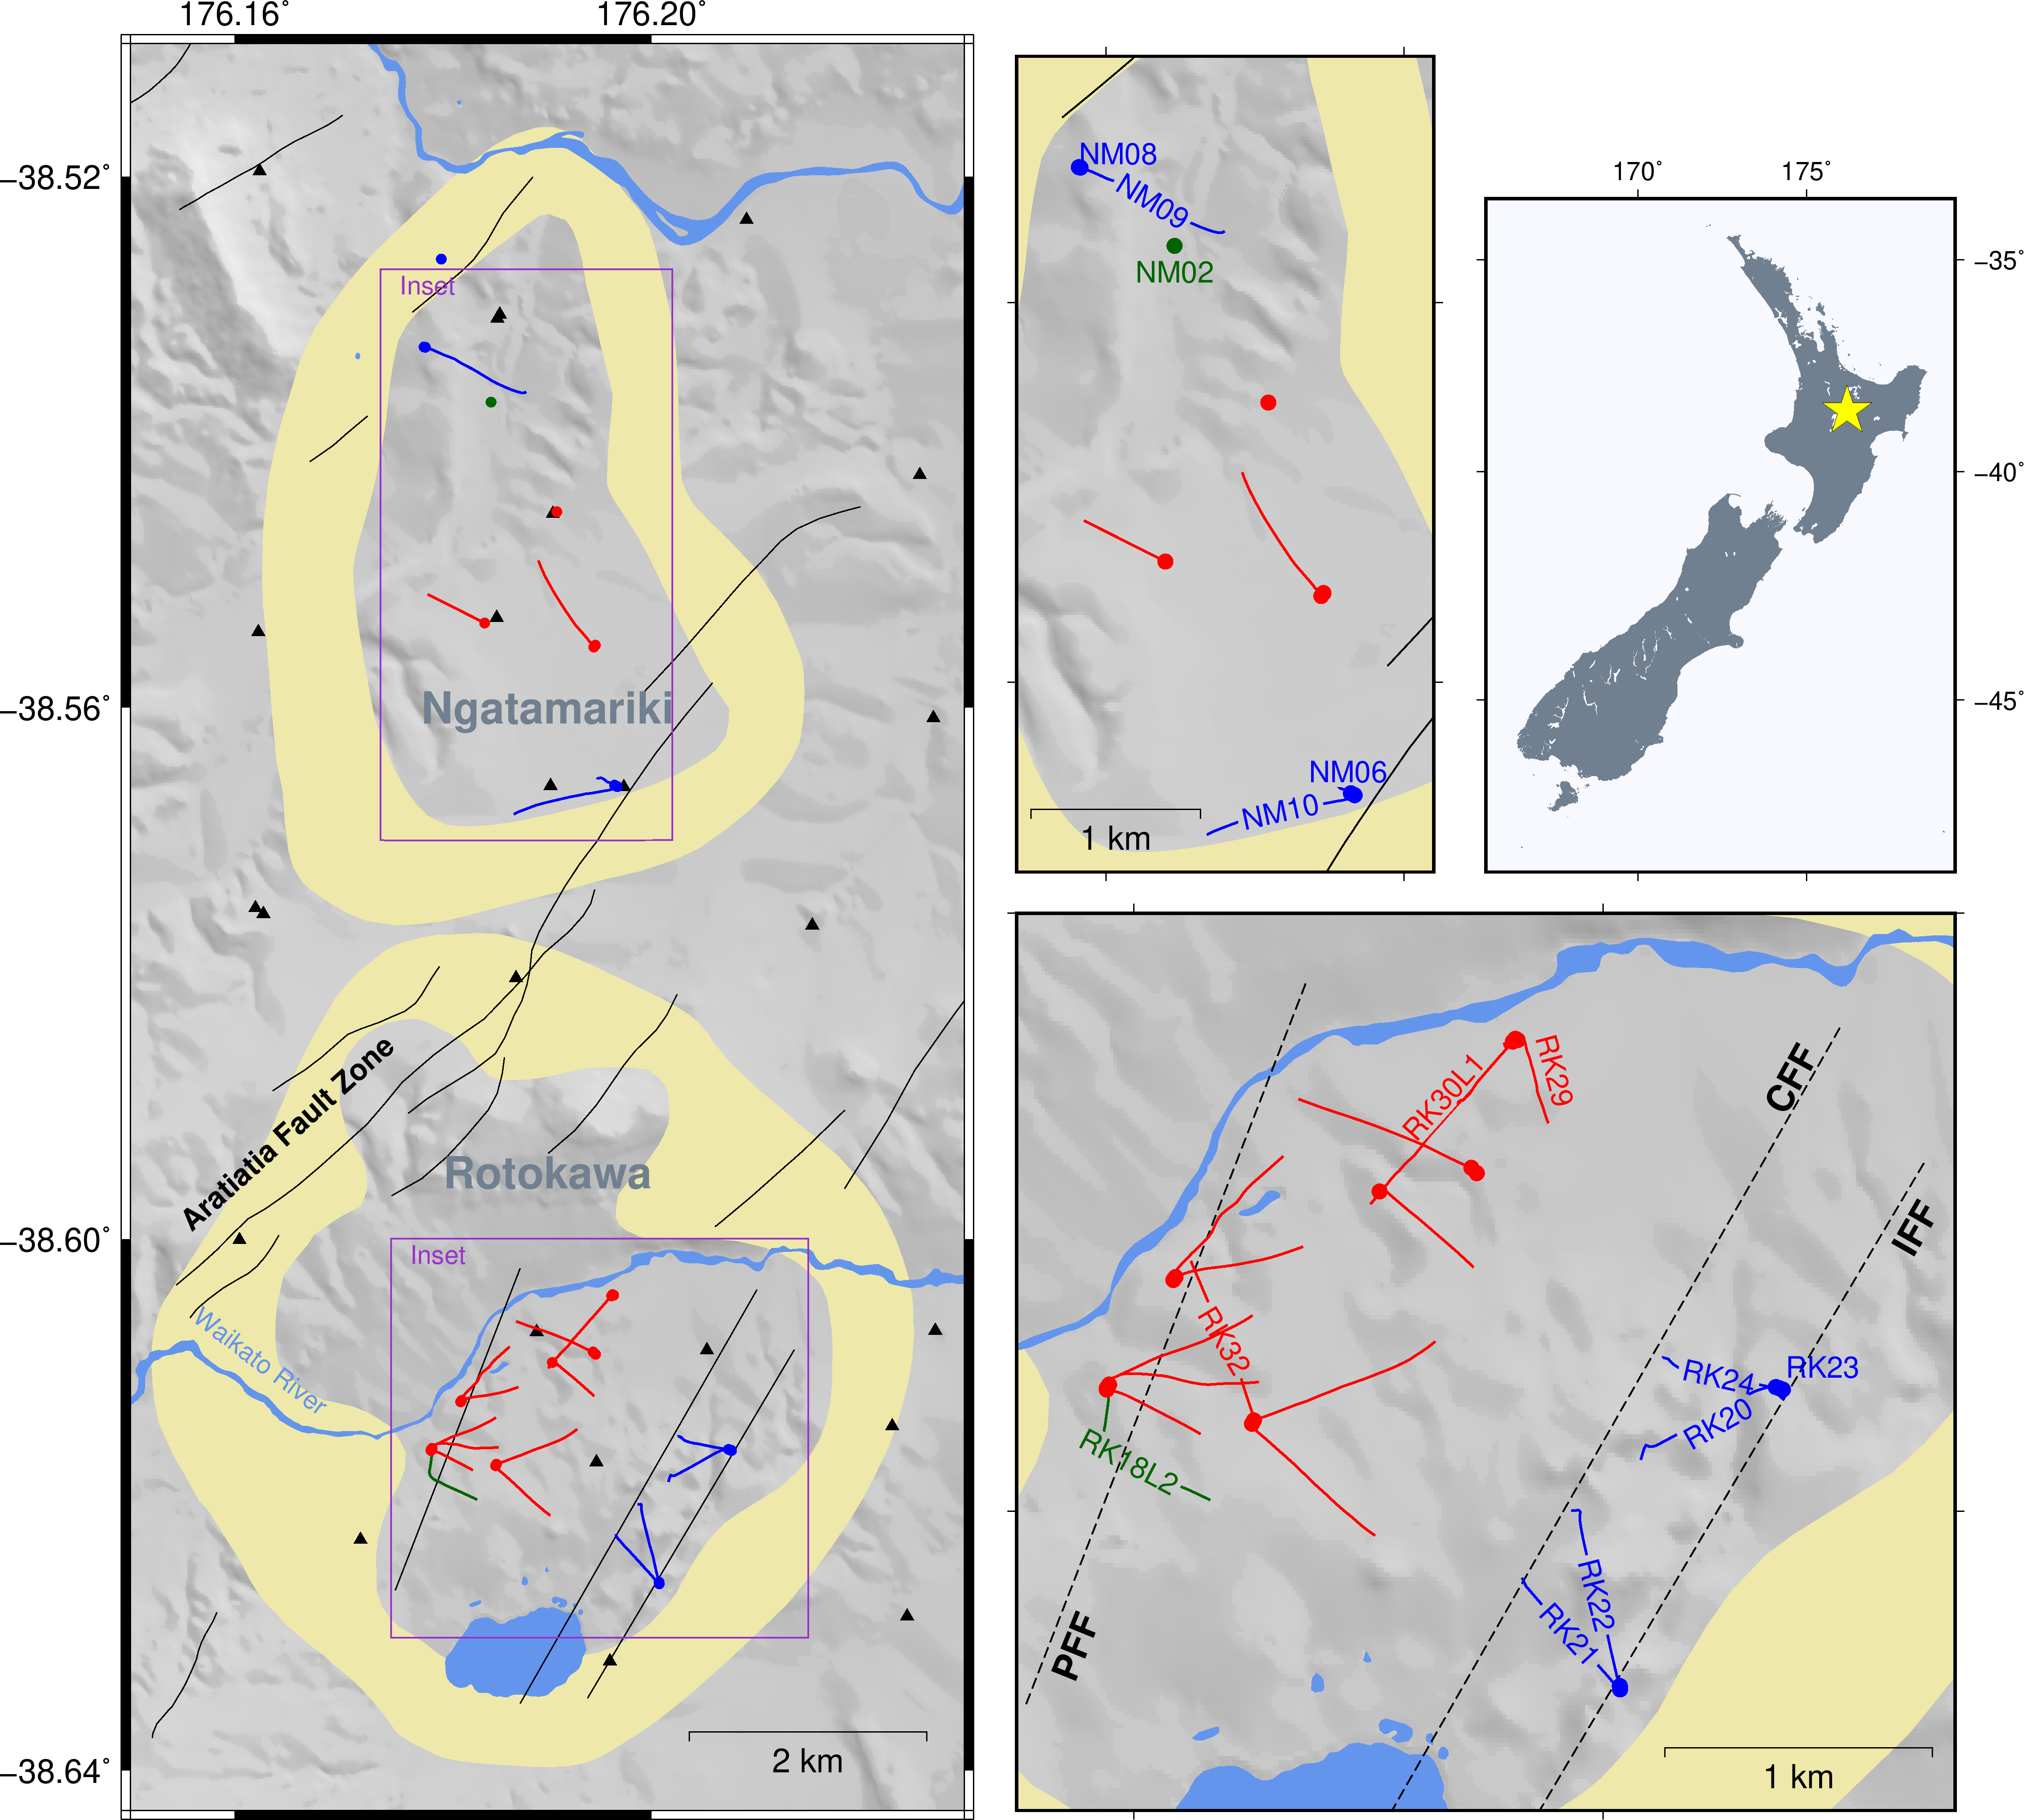
\includegraphics[width=1.00\columnwidth]{Chapter_5_FMs/figures/RotNga_overview/merc_RotNga_overview_struct}
\caption[Overview of the Ngatamariki and Rotokawa geothermal fields]{{
Overview map of the Ngatamariki and Rotokawa geothermal fields. Yellow polygons show the extend of each geothermal resource as defined by resistivity surveys \citep{Risk_2000,Boseley_2010}, black lines are mapped faults, and triangles are seismic stations used for this study. Within the fields, blue, red and green lines show the surface projection of injection, production and monitoring wells, respectively, with a circle indicating the location of the wellhead. Wells mentioned in the text are labeled in the inset panels. At Rotokawa, the modelled surface traces of the \acrfull{PFF}, \acrfull{CFF} and \acrfull{IFF} are plotted as dotted lines.
{\label{overview_Rot_Nga}}%
}}
\end{center}
\end{figure}\selectlanguage{english}

In this work we present a catalog of earthquake focal mechanisms solutions for both fields and use these catalogs to invert for the stress state. We attempt to address the resulting stress variations in space and time and comment on the potential relationships between power production (specifically fluid injection) and stress tensor variation. To our knowledge, this is the first study to use focal mechanism inversion to study stress state at a New Zealand geothermal field. However, the tectonic setting in the \acrshort{TVZ} is comparable to that at large geothermal fields elsewhere (e.g. The Geysers in northern California, USA) where extensive stress studies have been conducted using both high-quality focal mechanism inversions and coupled thermo-hydro-mechanical numerical simulations \citep[e.g.][]{Mart_nez_Garz_n_2013,Boyle_2014,Jeanne_2015tensor}. We refer to these studies to provide context for our results and suggest mechanisms for stress change in geothermal reservoirs in general.

\subsection{Stress changes at geothermal reservoirs}\label{stress_background}
In the last three decades, a number of workers have attempted to characterize the state of stress in geothermal reservoirs and determine the potential changes related to fluid injection and extraction activities \citep{oppenheimer1986extensional,feng1998microseismicity,sasaki2002determination,bohnhoff2004fault,Mart_nez_Garz_n_2013,Boyle_2014,Mart_nez_Garz_n_2014,Mart_nez_Garz_n_2017}. Although some of these studies were hampered by small amounts of data, the more recent works \citep[specifically][]{Mart_nez_Garz_n_2013,Boyle_2014,Mart_nez_Garz_n_2014,Mart_nez_Garz_n_2017} at The Geysers geothermal field in California were able to make use of large datasets of high-precision, well-constrained focal mechanisms ($n$\textgreater{6000} events) to invert for the principle stress axes in time and space.

Although starting from the same underlying dataset, \citet{Mart_nez_Garz_n_2013} and \citet{Boyle_2014} came to different conclusions from their stress inversion results. \citet{Boyle_2014} concluded that there was no discernible spatial deviation in the stress field related to injection\slash{extraction} activities at The Geysers, based on their observation that S$_{Hmax}$ was consistent both inside and outside of the reservoir, as well as at different depth intervals and spatial grid sizes. In contrast, \citet{Mart_nez_Garz_n_2013} determined that, at reservoir depths, They Geysers stress state is normal\slash{transtensional} and strike-slip\slash{transtensional} above and below. This is due to an apparent swapping of $\sigma_1$ and $\sigma_2$ dips at reservoir depths, leaving S$_{Hmax}$ unchanged (N15\textdegree{E}). It should be noted that, although \citet{Boyle_2014} concluded that power production activities had no effect on the stress state of the reservoir, their observations are not entirely inconsistent with those of \citet{Mart_nez_Garz_n_2013}, both of which show that S$_{Hmax}$ is unchanged throughout The Geysers.

Thermo-hydro-mechanical modeling of the stress-state response to injection at the Geysers \citep{Jeanne_2014,Jeanne_2015tensor} supports the interpretation of \citet{Mart_nez_Garz_n_2013}. They show that thermal contraction of the host rock at reservoir depths causes a variation in the dip of $\sigma_{1}$ at and below the depth of injection \citep{Jeanne_2015tensor}. This is because the injected fluid, which is much denser than the hot reservoir fluid, `sinks' to greater depths upon injection. This effect causes the cooled volume of the reservoir to take on a shape that is longer in the z (depth) direction than in the x or y direction, thereby reducing vertical stress more than the horizontal stresses. In their model, since $\sigma_{1}\approx{\sigma_{V}}$ at The Geysers (normal faulting regime), cooling reduction of $\sigma_{1}$ actually caused $\sigma_{1}$ and $\sigma_{2}$ (S$_{Hmax}$) to trade places after 7-8 months of injection, artificially inducing a strike-slip faulting regime within the reservoir \citep{Jeanne_2015tensor}. No such effect was observed when the same models were run in the absence of thermoelastic effects, indicating that these stress rotations are unique to injections where the temperature contrast between injected fluid and reservoir is high \citep{Jeanne_2015tensor}. 

These results likely apply directly to the development of the Ngatamariki and Rotokawa reservoirs, where the stress state and natural-state reservoir temperature are similar to The Geysers. 

\subsection{Fractures and stress state at Rotokawa and Ngatamariki}
At reservoir scale, structure at Ngatamariki and Rotokawa mirrors the NE-SW-striking trend of extensional faulting observed across the Taup\={o} Volcanic Zone. These NW- and SE-dipping antithetic structures accommodate the $\sim$5--15 mm/y of NW-SE regional extension \citep{Rowland_2004,Wallace_2004}. The only major structure to intersect both the Ngatamariki and Rotokawa reservoirs is the Aratiatia Fault Zone (Figure \ref{overview_Rot_Nga}). However, a number of other NE-SW structures of \textgreater{1} km in length have been inferred to exist within the fields \citep{wallis2013,Chambefort_2014}. Within the production and injection fields at Rotokawa, three major faults have been identified from geologic modeling of vertical offsets of well cuttings \citep{wallis2013}. From NW to SE these are the \acrfull{PFF}, \acrfull{CFF} and \acrfull{IFF} (Figure \ref{overview_Rot_Nga}).

If we consider the reservoirs at a scale of meters to 100s of meters, the orientation and extent of fracturing is mainly known through interpretation of borehole logs at selected wells (see Section \ref{data-methods}). At this scale, fracturing in the reservoirs exhibits the same NE-SW trend as the regional-scale faults. However, between wells and across both fields, the dominant dip of fracturing varies, likely controlled by the dip direction of the nearest large fault zone \citep{McNamara_2015}.

The TVZ is a zone of active extensional tectonics, with a stress state described by $\sigma_{1}\approx{\sigma_{V}}$ and S$_{Hmax}$ trending NE-SW \citep{Townend_2012}. Inversion of earthquake focal mechanisms has estimated the direction of S$_{Hmax}$ in the Central Taup\={o} Volcanic Zone to have an azimuth of $\sim$052--058\textdegree{} \citep{hurst2002earthquake,hurst2008characteristics}. Other estimates of the direction of S$_{Hmax}$ have been made from the orientation of drilling induced tensile fractures and other induced structures observed in borehole image logs at Rotokawa \citep{McNamara_2015}. For wells RK18L2, RK32 and RK30L1, estimates of S$_{Hmax}$ ranged from 025--049\textdegree{} \citep{McNamara_2015}. \citet{davidson_2012} also attempted to estimate the magnitudes of the principle stress components at Rotokawa but were hampered by a number of complexities with the data, including complex lateral variations in overburden and a lack of observed borehole breakout \citep{McNamara_2015}. No magnitude was estimated for S$_{Hmax}$ due to the lack of observed breakout, which \citet{davidson_2012} suggest was the result of the temperature range between drilling fluid and reservoir rock, suppressing the expansion of the borehole necessary to produce breakout. They were able to demonstrate that $\sigma_{V}$ and S$_{Hmin}$ ($\sigma_{3}$) at reservoir levels ($\sim$1100 m bsl) in Rotokawa vary laterally by up to 5 MPa over scales of less than a kilometer, similar to results presented for the Coso geothermal field in California \citep[e.g.][]{davidson_2012,blake2011crustal}.

\section{Data and methods}\label{data-methods}
\subsection{Earthquake catalog}
The earthquake catalog analyzed here was provided by GNS Science under contract with Mercury NZ, Ltd. Earthquake detection and location were conducted automatically using the \textit{SeisComP3} software package \citep{Weber2007}. We then revised the entire catalog manually, adjusting arrival times where warranted and picking P-wave first arrival polarities where possible. After removing all events with fewer than five polarity picks, 982 events remained. These events were separated into catalogs for each field (205 events for Ngatamariki, 777 for Rotokawa) and then incorporated into a large catalog of matched-filter detected events (\citet[described in detail by][]{j2019}). Finally, we relocated the entire catalog using the double-difference relocation program \textit{GrowClust} \citep{Trugman_2017}.

\subsection{Focal Mechanism Determination}\selectlanguage{english}
To calculate the focal mechanism solutions for this study, we used the Bayesian approach of \citet{Walsh_2009}, which allows the us to incorporate known uncertainties of the input parameters, specifically in hypocentral location and polarity picking error. Solutions were calculated using only manually-picked P-wave polarities, so long as a minimum of five picks were made per event. We calculated a total of 205 focal mechanism solutions at Ngatamariki and 777 at Rotokawa (Figures \ref{542095} and \ref{817909}). There are a median of seven polarity picks per event and an average standard deviation of the strike/dip/rake of 31.4\textdegree{}.

\begin{figure}[h!]
\begin{center}
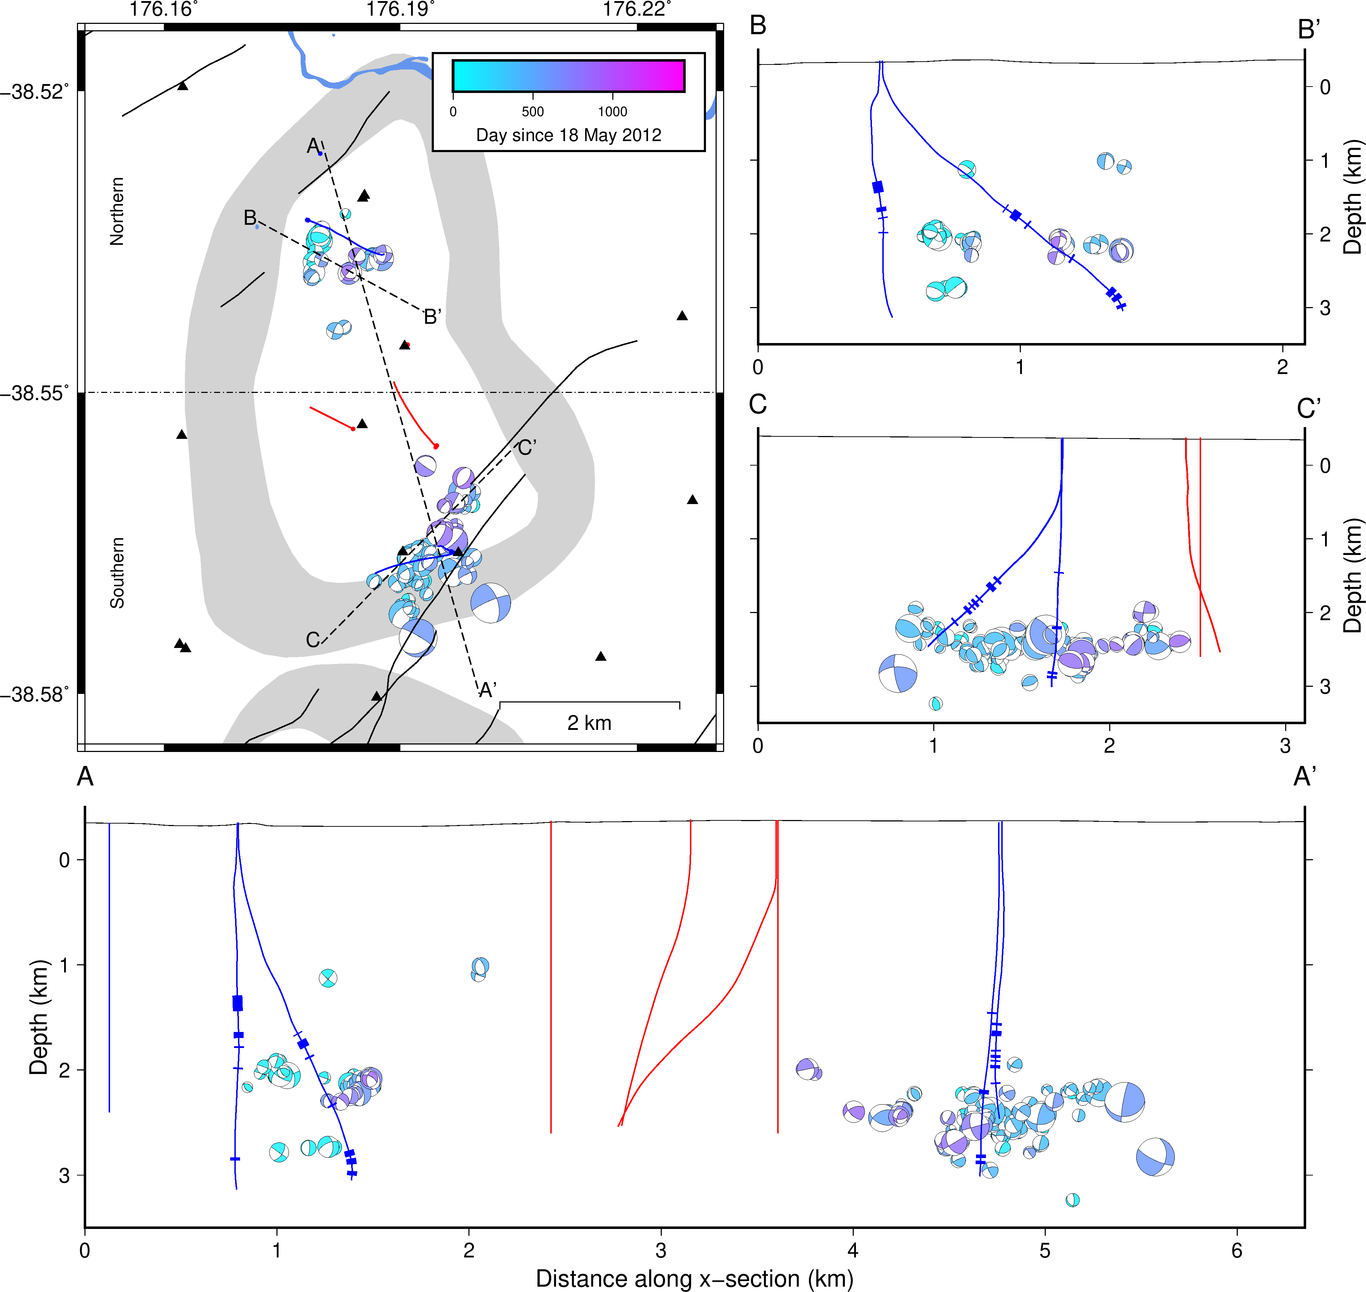
\includegraphics[width=1.00\columnwidth]{Chapter_5_FMs/figures/merc_Nga_GC_focmecs/merc_Nga_GC_focmecs}
\caption[Ngatamariki focal mechanism solutions]{{
All calculated focal mechanisms for Ngatamariki from May 2012 until
November 2015. Grey polygons show the resistivity boundaries for
Ngatamariki (to the north) and Rotokawa (to the south). Black lines
indicate active faults from the GNS Active Fault Database \citep{AFDB} with the inferred orientation of the \acrshort{IFF} and \acrshort{CFF} drawn in bold and labeled. Red, blue and green lines indicate production, injection and monitoring wells. Focal mechanisms are colored by the
date of occurrence, with earlier events colored blue and later events
colored pink. Focal mechanisms have been reprojected in each
cross-section view to show ``back-hemisphere'' projections (i.e. the
hemisphere ``behind'' the panel). Each cross section shows only the
events within 1.5 km of the plane. Black triangles show the locations of
seismic stations.
{\label{542095}}%
}}
\end{center}
\end{figure}\selectlanguage{english}

As expected in the extensional TVZ, focal mechanisms at both fields show predominantly oblique normal faulting with subvertical P-axes. B-axis plunges are well distributed at Ngatamariki, showing no preference between pure normal and pure strike-slip faulting, whereas at Rotokawa, faulting is mostly normal with a minor oblique component (Figure \ref{FMC}). The mode of faulting at both fields appears to be unrelated to the hypocentral depth (Figure \ref{FMC}). 

\begin{figure}[h!]
\begin{center}
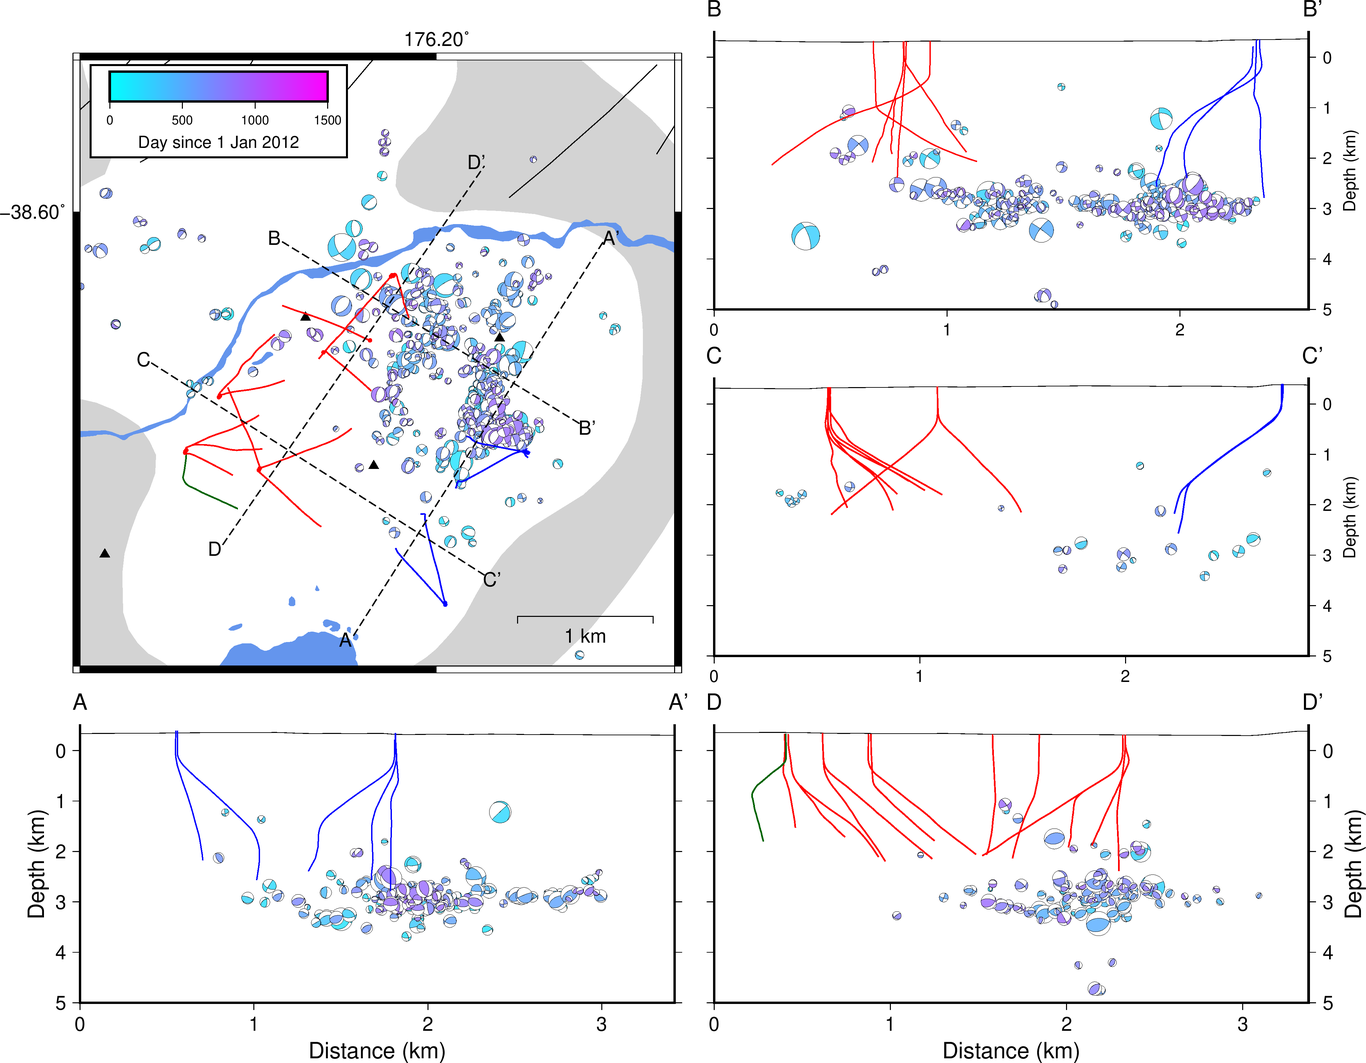
\includegraphics[width=1.00\columnwidth]{Chapter_5_FMs/figures/merc_Rot_GC_focmecs/merc_Rot_GC_focmecs}
\caption[Rotokawa focal mechanism solutions]{{
All calculated focal mechanisms for Rotokawa from May 2012 until
November 2015. The grey polygon shows the resistivity boundaries for
Rotokawa. Black lines indicate active faults from the GNS Active Fault
Database \citep{AFDB}, red lines indicate
production wells, blue lines indicate injection wells and the green line
is a reservoir monitoring well. Focal mechanisms are colored by the date
of occurrence, with earlier events colored blue and later events colored
pink. Focal mechanisms have been reprojected in each cross-section view
to show ``back-hemisphere'' projections (i.e. the hemisphere ``behind''
the panel). Each cross section shows only the events within 1.5 km of
the plane. Black triangles show the locations of seismic stations.
{\label{817909}}%
}}
\end{center}
\end{figure}

\begin{figure}[h!]
\begin{center}
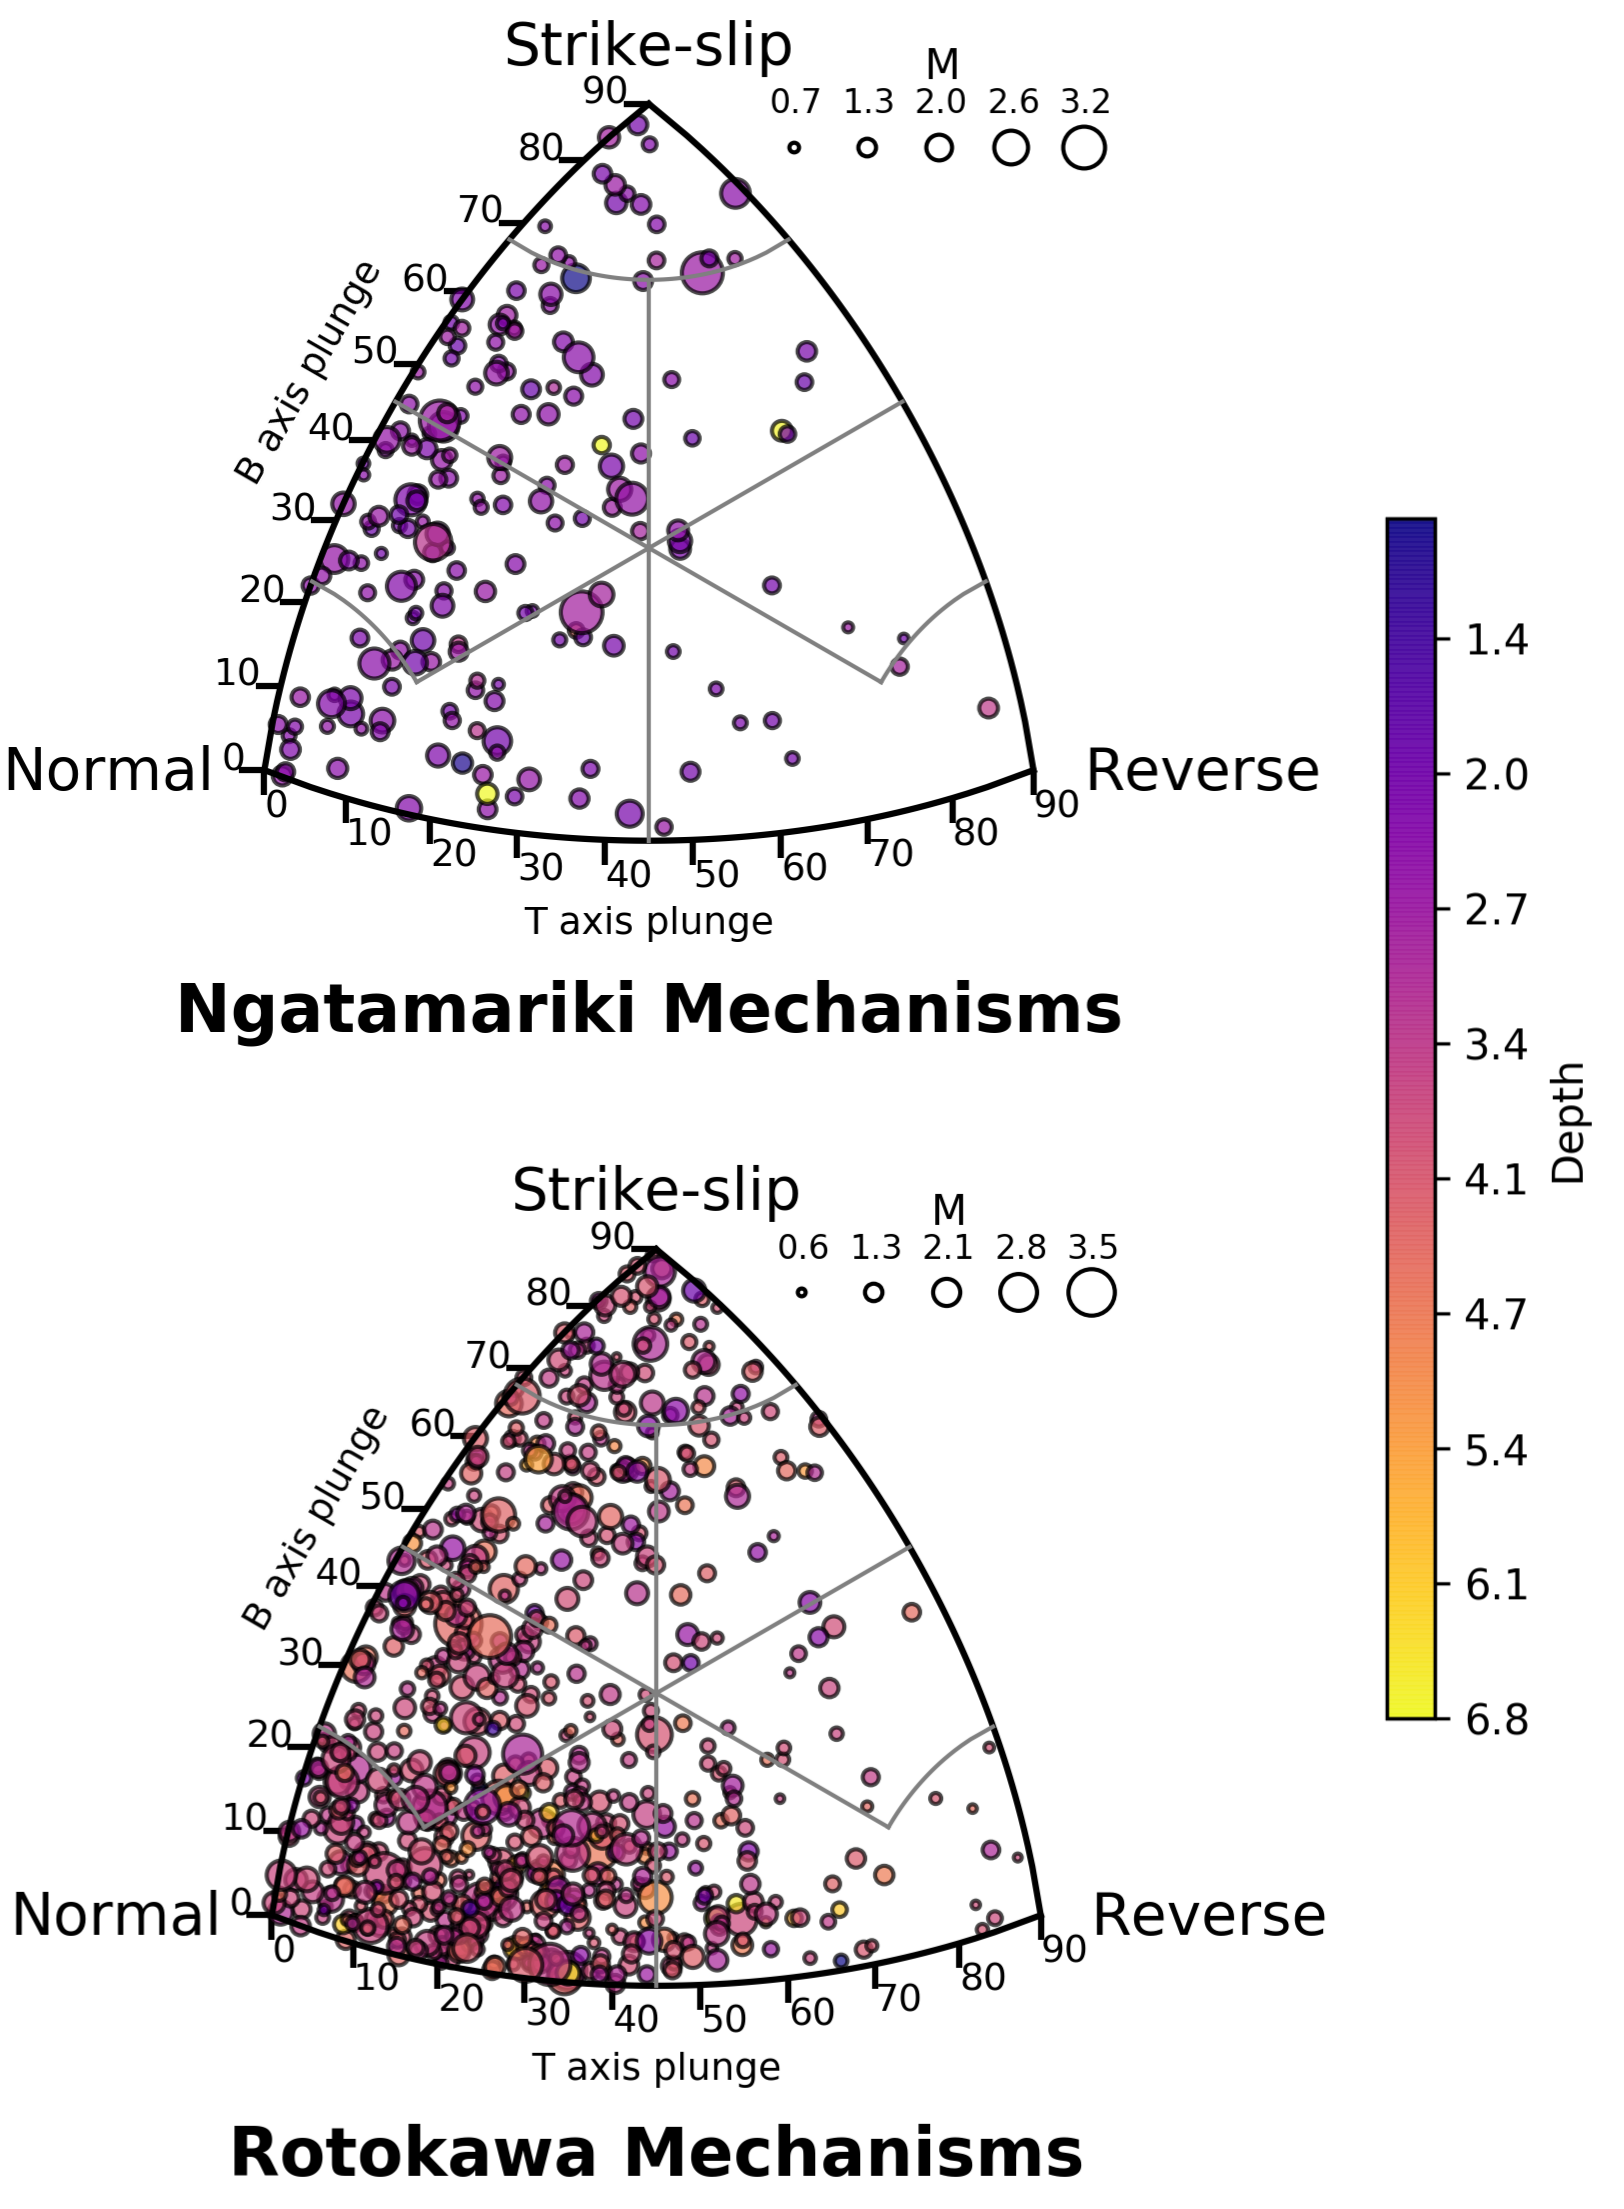
\includegraphics[width=0.8\columnwidth]{Chapter_5_FMs/figures/FMC_plots/Merc_ALL_FMC_crop}
\caption[Kaverina diagrams of focal mechanism solutions at both fields]{{
Kaverina diagrams \citep{kaverina1996global,alvarez2014fmc} showing the kinematics for all focal mechanisms at Ngatamariki (top) and Rotokawa (bottom) based on the plunge of the B (null) and T axes for each event. Circles are scaled by magnitude and colored by depth.
{\label{FMC}}%
}}
\end{center}
\end{figure}

\subsection{K-means Clustering}
In order to investigate the spatial variation in the stress parameters at Rotokawa and Ngatamariki, we employ a `kmeans' clustering technique \citep{hartigan1975clustering}, based on the euclidian distances between all event pairs in the catalog. It is well known that the `kmeans' algorithm does not yield a unique solution to this clustering problem \citep[as noted by][]{Townend_2012}, but visual inspection of the results shows that no clusters violate logical divisions in the hypocenter distribution (across inferred faults, for example). We therefore have no reason to suspect that any particular cluster of samples multiple stress regimes, although this cannot be ruled out.

We divide the focal mechanisms at Ngatamariki (Figures \ref{542095}) into $k=$10 clusters and at Rotokawa (Figure \ref{817909}) into $k=$30 clusters, retaining only those clusters with 20 events or more. We performed the clustering over a range of $k$ values ($k=$5--30 at Ngatamariki; $k=$18--60 at Rotokawa) before selecting the value that maximized the number of groups at either field.

\subsection{Stress Inversion}
For each of the clusters established above, we inverted for the three principle stress axes ($\sigma_{1,2,3}$) and the stress ratio, $\nu$:
\begin{equation}
    \nu = \frac{\sigma_{1} - \sigma_{2}}{\sigma_{1} - \sigma_{3}}
\end{equation}
using the approach of \citet{Arnold_2007}. This approach allows us to readily incorporate the uncertainties in the focal mechanism parameters (strike/dip/rake) calculated using the approach detailed above and outputs a PDF of $\sigma_{1,2,3}$ and $\nu$. These can then be incorporated into the transformation of \citet{Lund_2007}, which returns an estimate of S$_{Hmax}$ for non-trivial cases where one principle stress is not vertical.

\section{Results}\label{results}
\subsection{Stress inversions}
\subsubsection{Ngatamariki}
At Ngatamariki, kmeans clustering for $k$=10 yielded five clusters of 20 events or greater (Figure \ref{nga_kmeans}), two in the north and three in the south. In the north, Cluster 2 is located nearest to injection well NM08 and contains mostly events that occurred during NM08 stimulation \citep{j2019}, while Cluster 6 includes events occurring adjacent to injection well NM09 (Figure \ref{nga_kmeans}).

The southern clusters, (4, 1 and 9 from the SW to NE, respectively), run along the strike of the Aratiatia Fault Zone with Cluster 1 centered at vertical injection well NM06 (Figure \ref{nga_kmeans}).

% Ngatamariki clusters fig
\begin{sidewaysfigure}[p]
\begin{center}
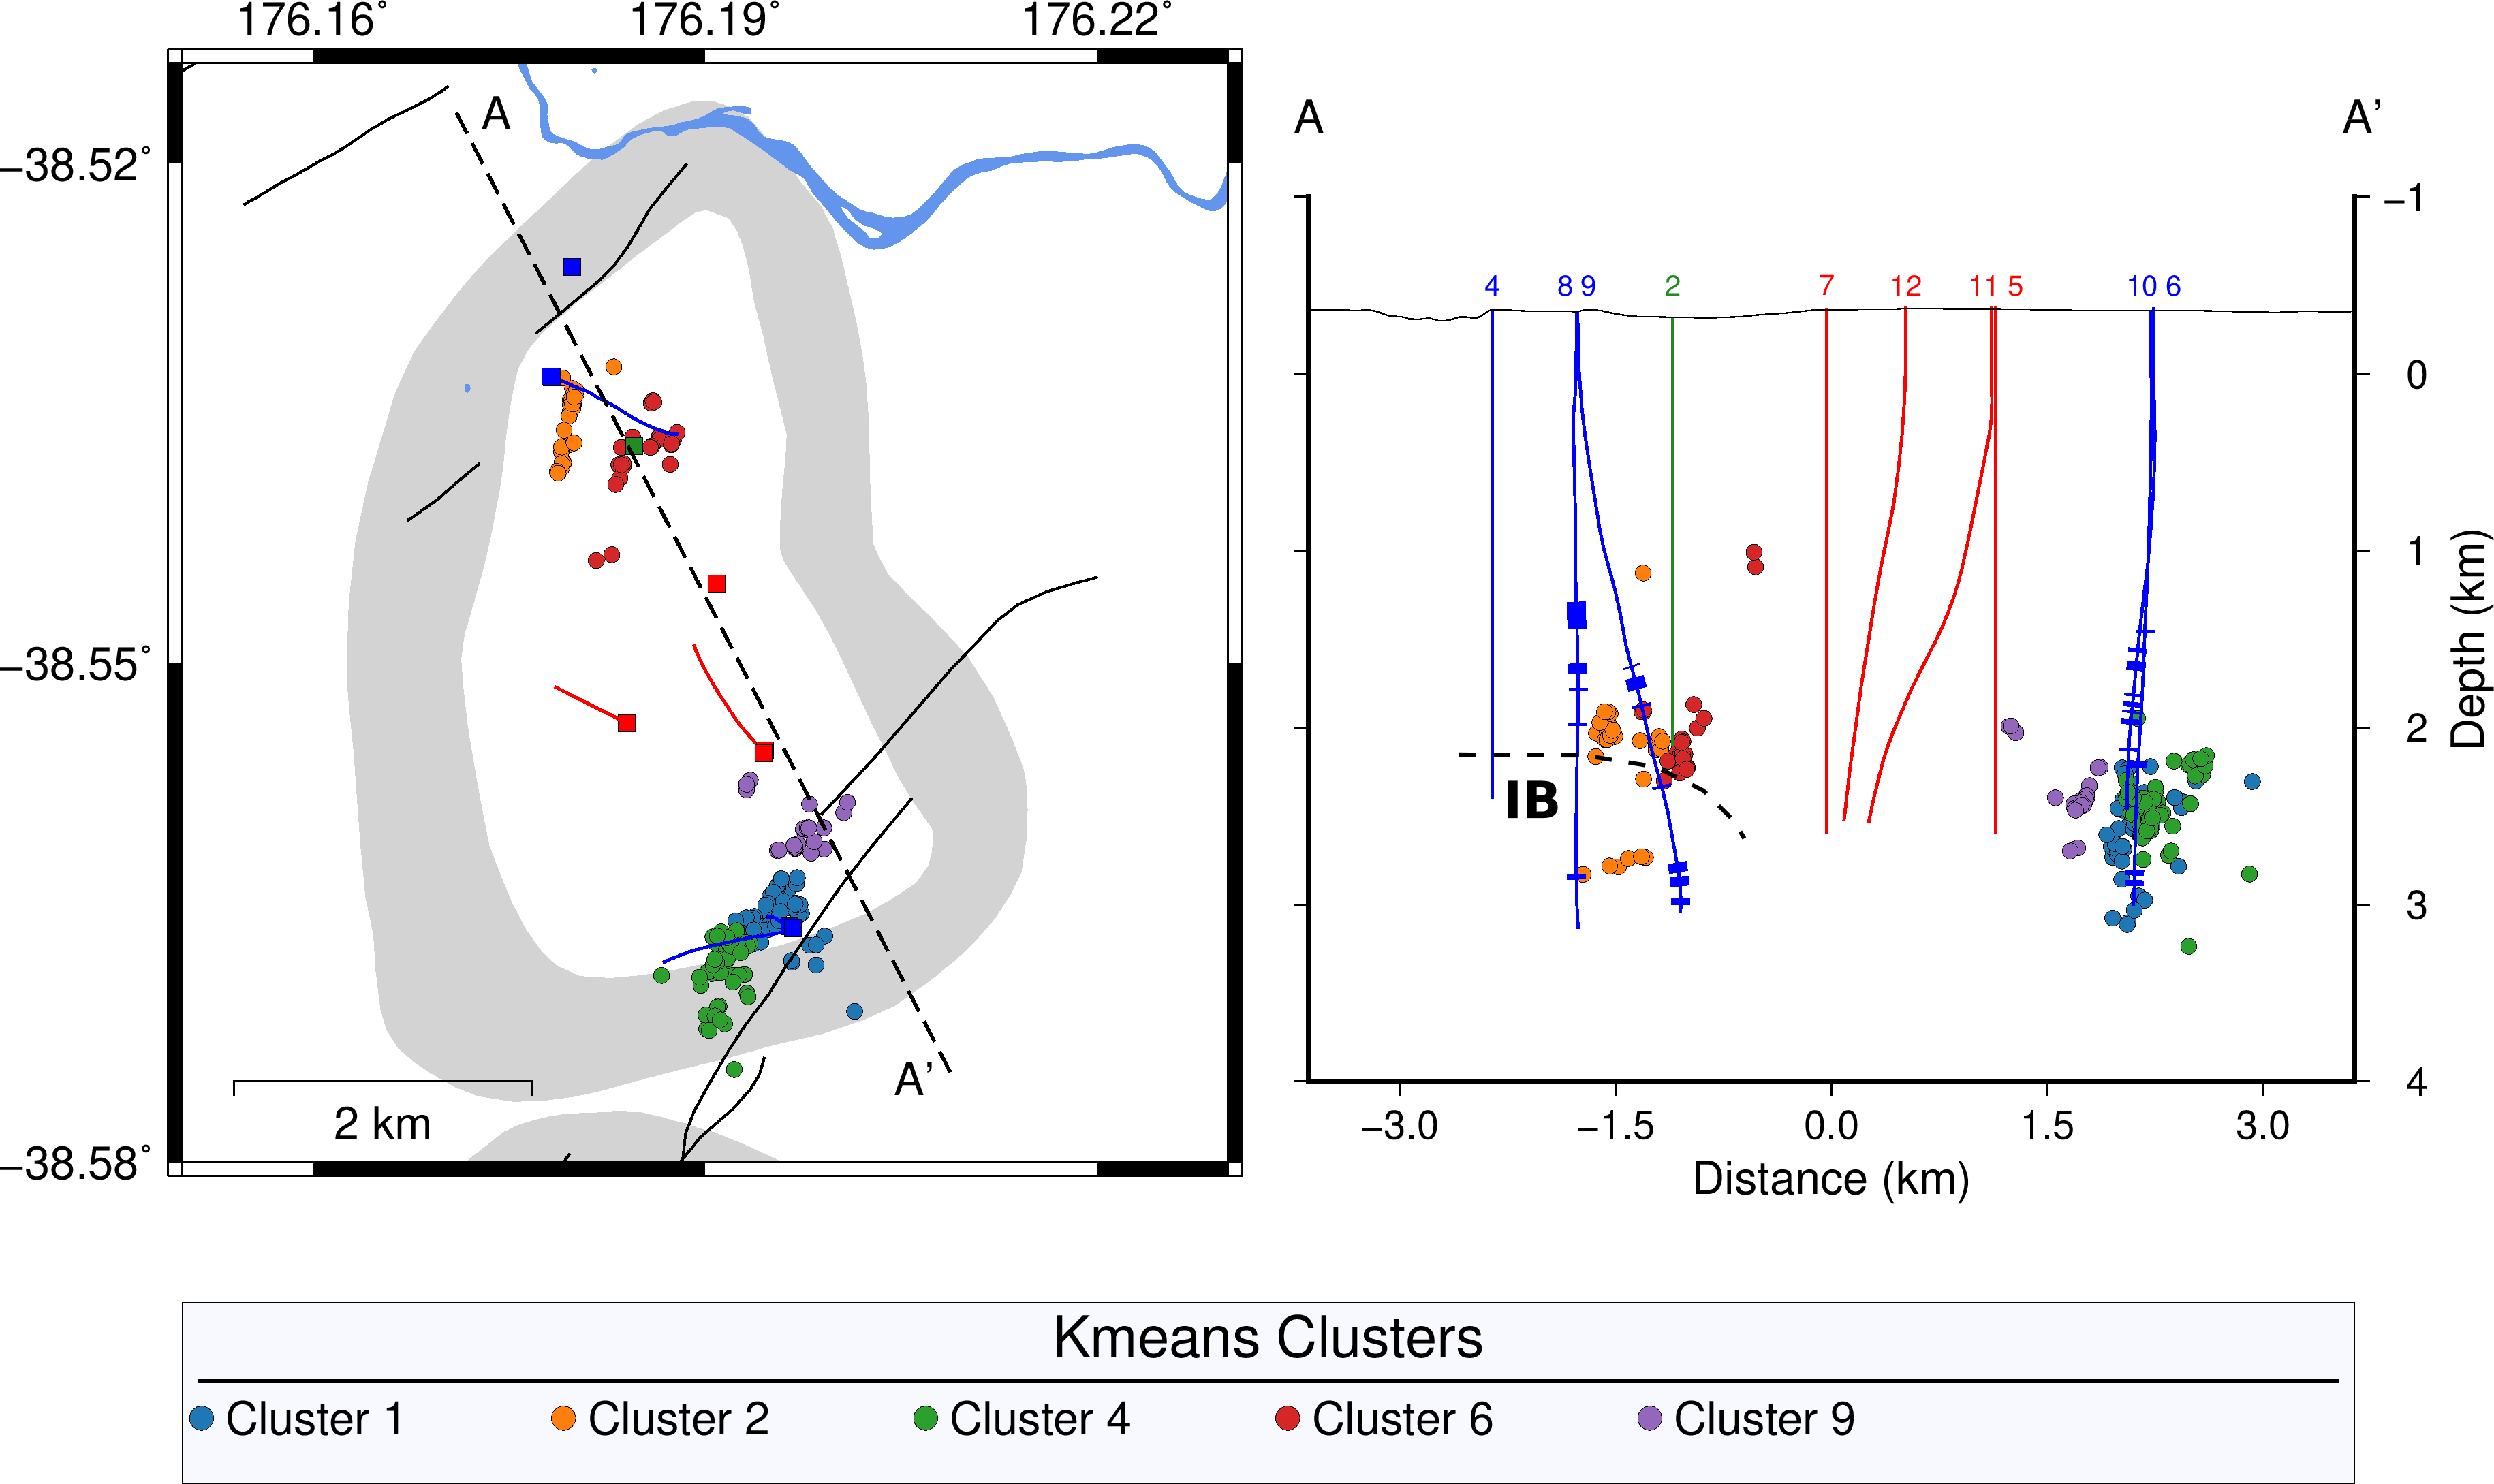
\includegraphics[width=0.8\textwidth,height=\textheight,keepaspectratio]{Chapter_5_FMs/figures/merc_Nga_GC_kmeans_10_GC_12-2-18/merc_Nga_kmeans_10_GC_12-2-18_intrusive}
\caption[Ngatamariki kmeans clusters]{{
Ngatamariki kmeans clusters ($k$=10) with 20 events or more. Red, blue and green lines represent production, injection and monitoring wells, respectively where the line is the well track and the square is the wellhead. The gray shaded area shows the resistivity boundary for the field \citep{Boseley_2010} and black lines indicate active faults \citep{AFDB}. In cross section, the dotted line at the bottom of the northern injection wells represents the top of the intrusive body (labeled `IB') as defined by well cuttings.
{\label{nga_kmeans}}%
}}
\end{center}
\end{sidewaysfigure}\selectlanguage{english}

\citep[][submitted]{j2019} performed stress inversions at Ngatamariki on a subset of the focal mechanisms analyzed here. The events they analyzed occurred during the \gls{stimulation} and completion testing of wells NM08, NM09 and NM10 in 2012-2013. They found that the stress state in southern Ngatamariki to be normal, with $\sigma_{1}\approx{\sigma_{V}}$ and S$_{Hmax}$ trending NE-SW at $\sim$045\textdegree{}. However, in the northern injection zone they found the stress regime to be inconsistent with regional normal faulting. There $\sigma_{1}$ dipped to the NE at $\sim$30\textdegree{} and $\sigma_{2}$\slash{}$\sigma_{3}$ formed a girdle, indicating a high stress ratio ($\nu$\textgreater{0.8}), where their respective orientations were difficult to distinguish. The discrepancy between the stress states in the northern and southern injection fields was attributed to the emplacement of a tonalite intrusive body in northern Ngatamariki, which may have significantly deviated the stress state.

We find a similar trend to \citep[][submitted]{j2019} when including all focal mechanisms from 2012-2015 (an increase in the number of focal mechanisms from 86 to 205) (Figure \ref{838980}). The additional events do not change the results of the inversions in southern Ngatamariki compared to the previous study, and a normal faulting regime still prevails. The three southern clusters (4, 1 and 9) progress along strike of the Aratiatia Fault Zone from near injection well NM10 in the southwest to past injection well NM06 in the northeast. There is little variation between the three inversions for these clusters. For each, $\sigma_{1}\approx{\sigma{_V}}$, S$_{Hmax}$ is oriented $\sim$045\textdegree and the stress ratio is low, $\nu=$0.3--0.4.

In the north, the stress state for Cluster 2 is unsurprisingly similar to the results presented by \citep[][submitted]{j2019}, given that most of the events in this cluster are common between the two datasets. Cluster 6 includes only events that have yet to be used for stress inversion. While Clusters 2 and 6 are only 300--400 m apart, the inversions reveal distinct stress states. In Cluster 2 $\sigma_{1}$ dips $\sim$30\textdegree{} at $\sim$020\textdegree{}, while it dips $\sim$51\textdegree{} at $\sim$090\textdegree{} in Cluster 6, forming a girdle with $\sigma_{2}$, indicating a stress ratio, $\nu$ approaching zero.

% Ngatamariki inversions fig
\begin{figure}[h!]
\begin{center}
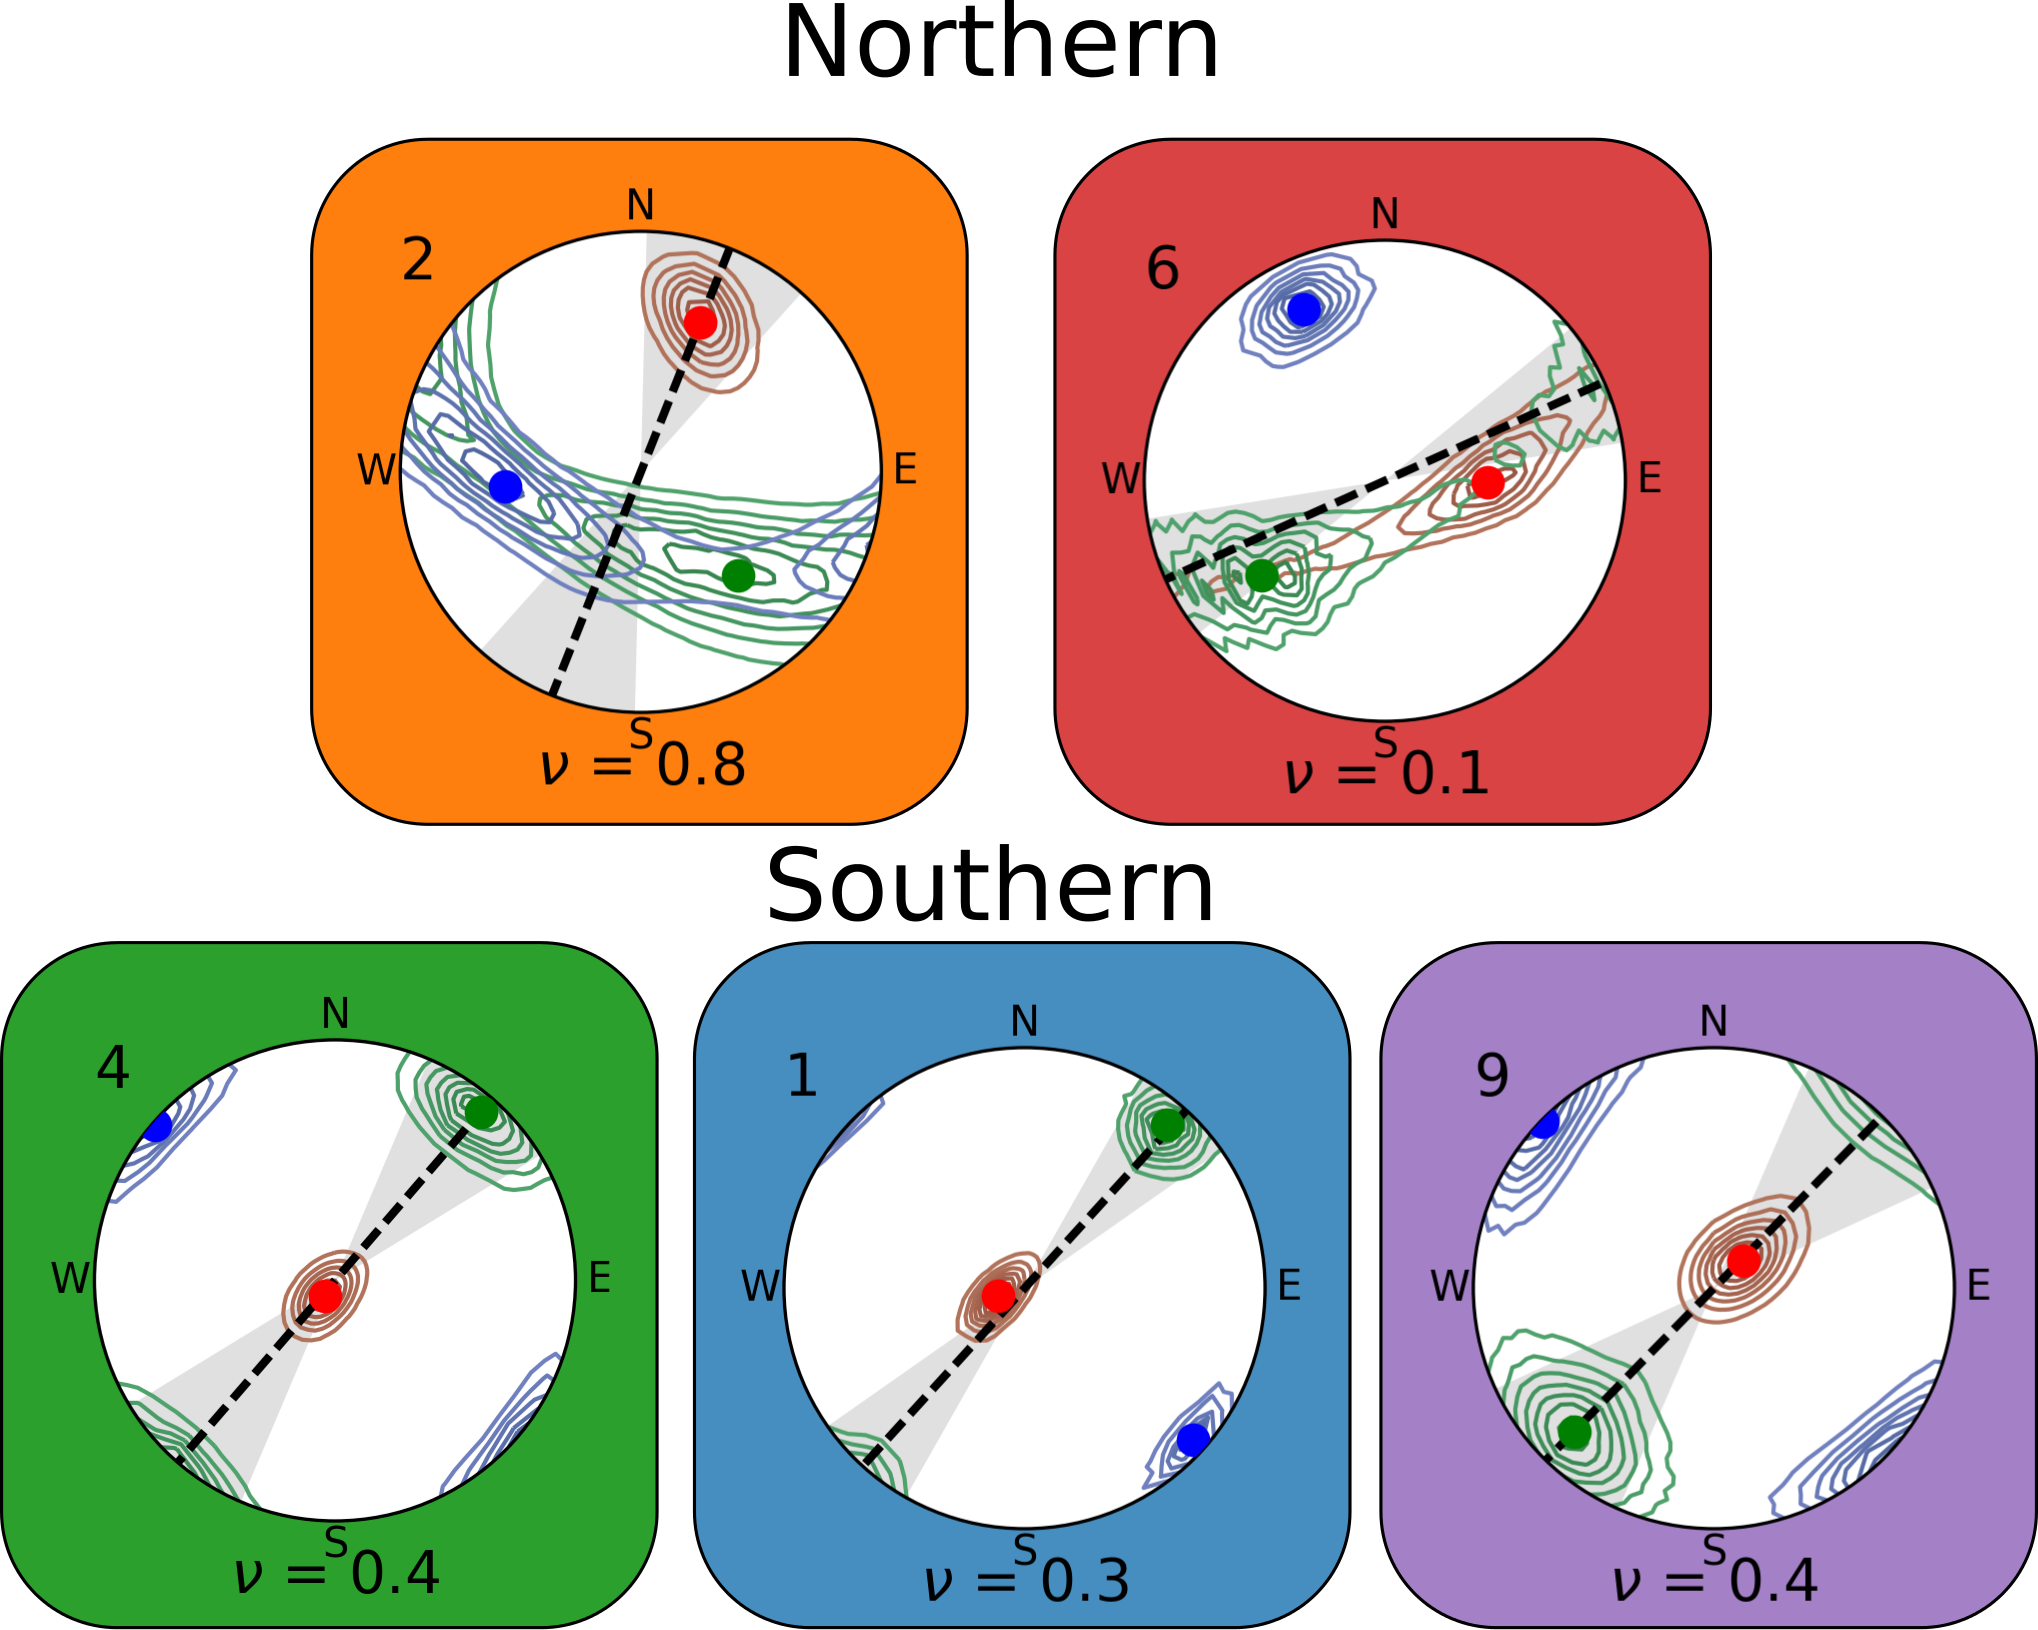
\includegraphics[width=0.98\columnwidth]{Chapter_5_FMs/figures/Nga_kmeans_inversion_10/Nga_temps_GC_dets_kmeans_10_transparent_colored}
\caption[Ngatamariki stress inversions from kmeans clusters]{{
Lower hemisphere stereonets representing the stress inversion results for each k-means cluster shown in Figure~{\ref{nga_kmeans}}. Red corresponds to $\sigma_{1}$, green to $\sigma_{2}$ and blue to $\sigma_{3}$, where the filled circle represents the maximum likelihood axis and the contours represent the shape of the PDF for that axis. The black dotted line shows the direction of maximum horzontal compressive stress (S$_{Hmax}$) for which the gray shaded bowtie shows the 90\% confidence region. Each plot is annotated below with the calculated stress ratio, $\nu$. Stereonet backgrounds are colored-coded to match the corresponding cluster in Figure~{\ref{nga_kmeans}}.
{\label{838980}}%
}}
\end{center}
\end{figure}

\subsubsection{Rotokawa}
At Rotokawa, the hypocenters for the focal mechanisms shown in Figure \ref{817909} reveal the same two NE-SW striking structures discussed in Chapter 4, which we continue to interpret as being the \acrfull{CFF} and \acrfull{IFF} from west to east, respectively. As these structures are known to act as cross-strike barriers to fluid flow, we choose to divide the reservoir into distinct `compartments' bounded by these structures (Figure \ref{878143}). Our chosen kmeans clustering parameter, $k$=30, produced 14 clusters, each containing a minimum of 20 focal mechanism observations. We then group these clusters into compartments as follows:

\begin{itemize}
\item{The western compartment (light green, Figures \ref{878143} and \ref{434168}), contains all clusters northwest of the \acrshort{IFF} and southeast of the \acrshort{CFF}. These are Clusters 7, 2, 9, 12 and 17, shown in Figure \ref{434168}}
\item{The southeastern compartment (pink, Figures \ref{878143} and \ref{434168}), contains clusters southeast of the \acrshort{IFF} and south of the cross-strike structure inferred from the offset in focal mechanism locations along strike of the \acrshort{IFF}. These are Clusters 0, 3, 25, 13, 14, and 15, shown in Figure \ref{434168}}
\item{The northeastern compartment (coral, Figures \ref{878143} and \ref{434168}), contains the remainder of the clusters southeast of the \acrshort{IFF} (Clusters 10 and 23, Figure \ref{434168}).}
\item{The final cluster, Cluster 28, is located just inside the northern production field. We infer the centroid of this cluster to be outside the bounds of the compartments described above.}
\end{itemize}

% Rotokawa clusters fig
\begin{sidewaysfigure}[p]
\begin{center}
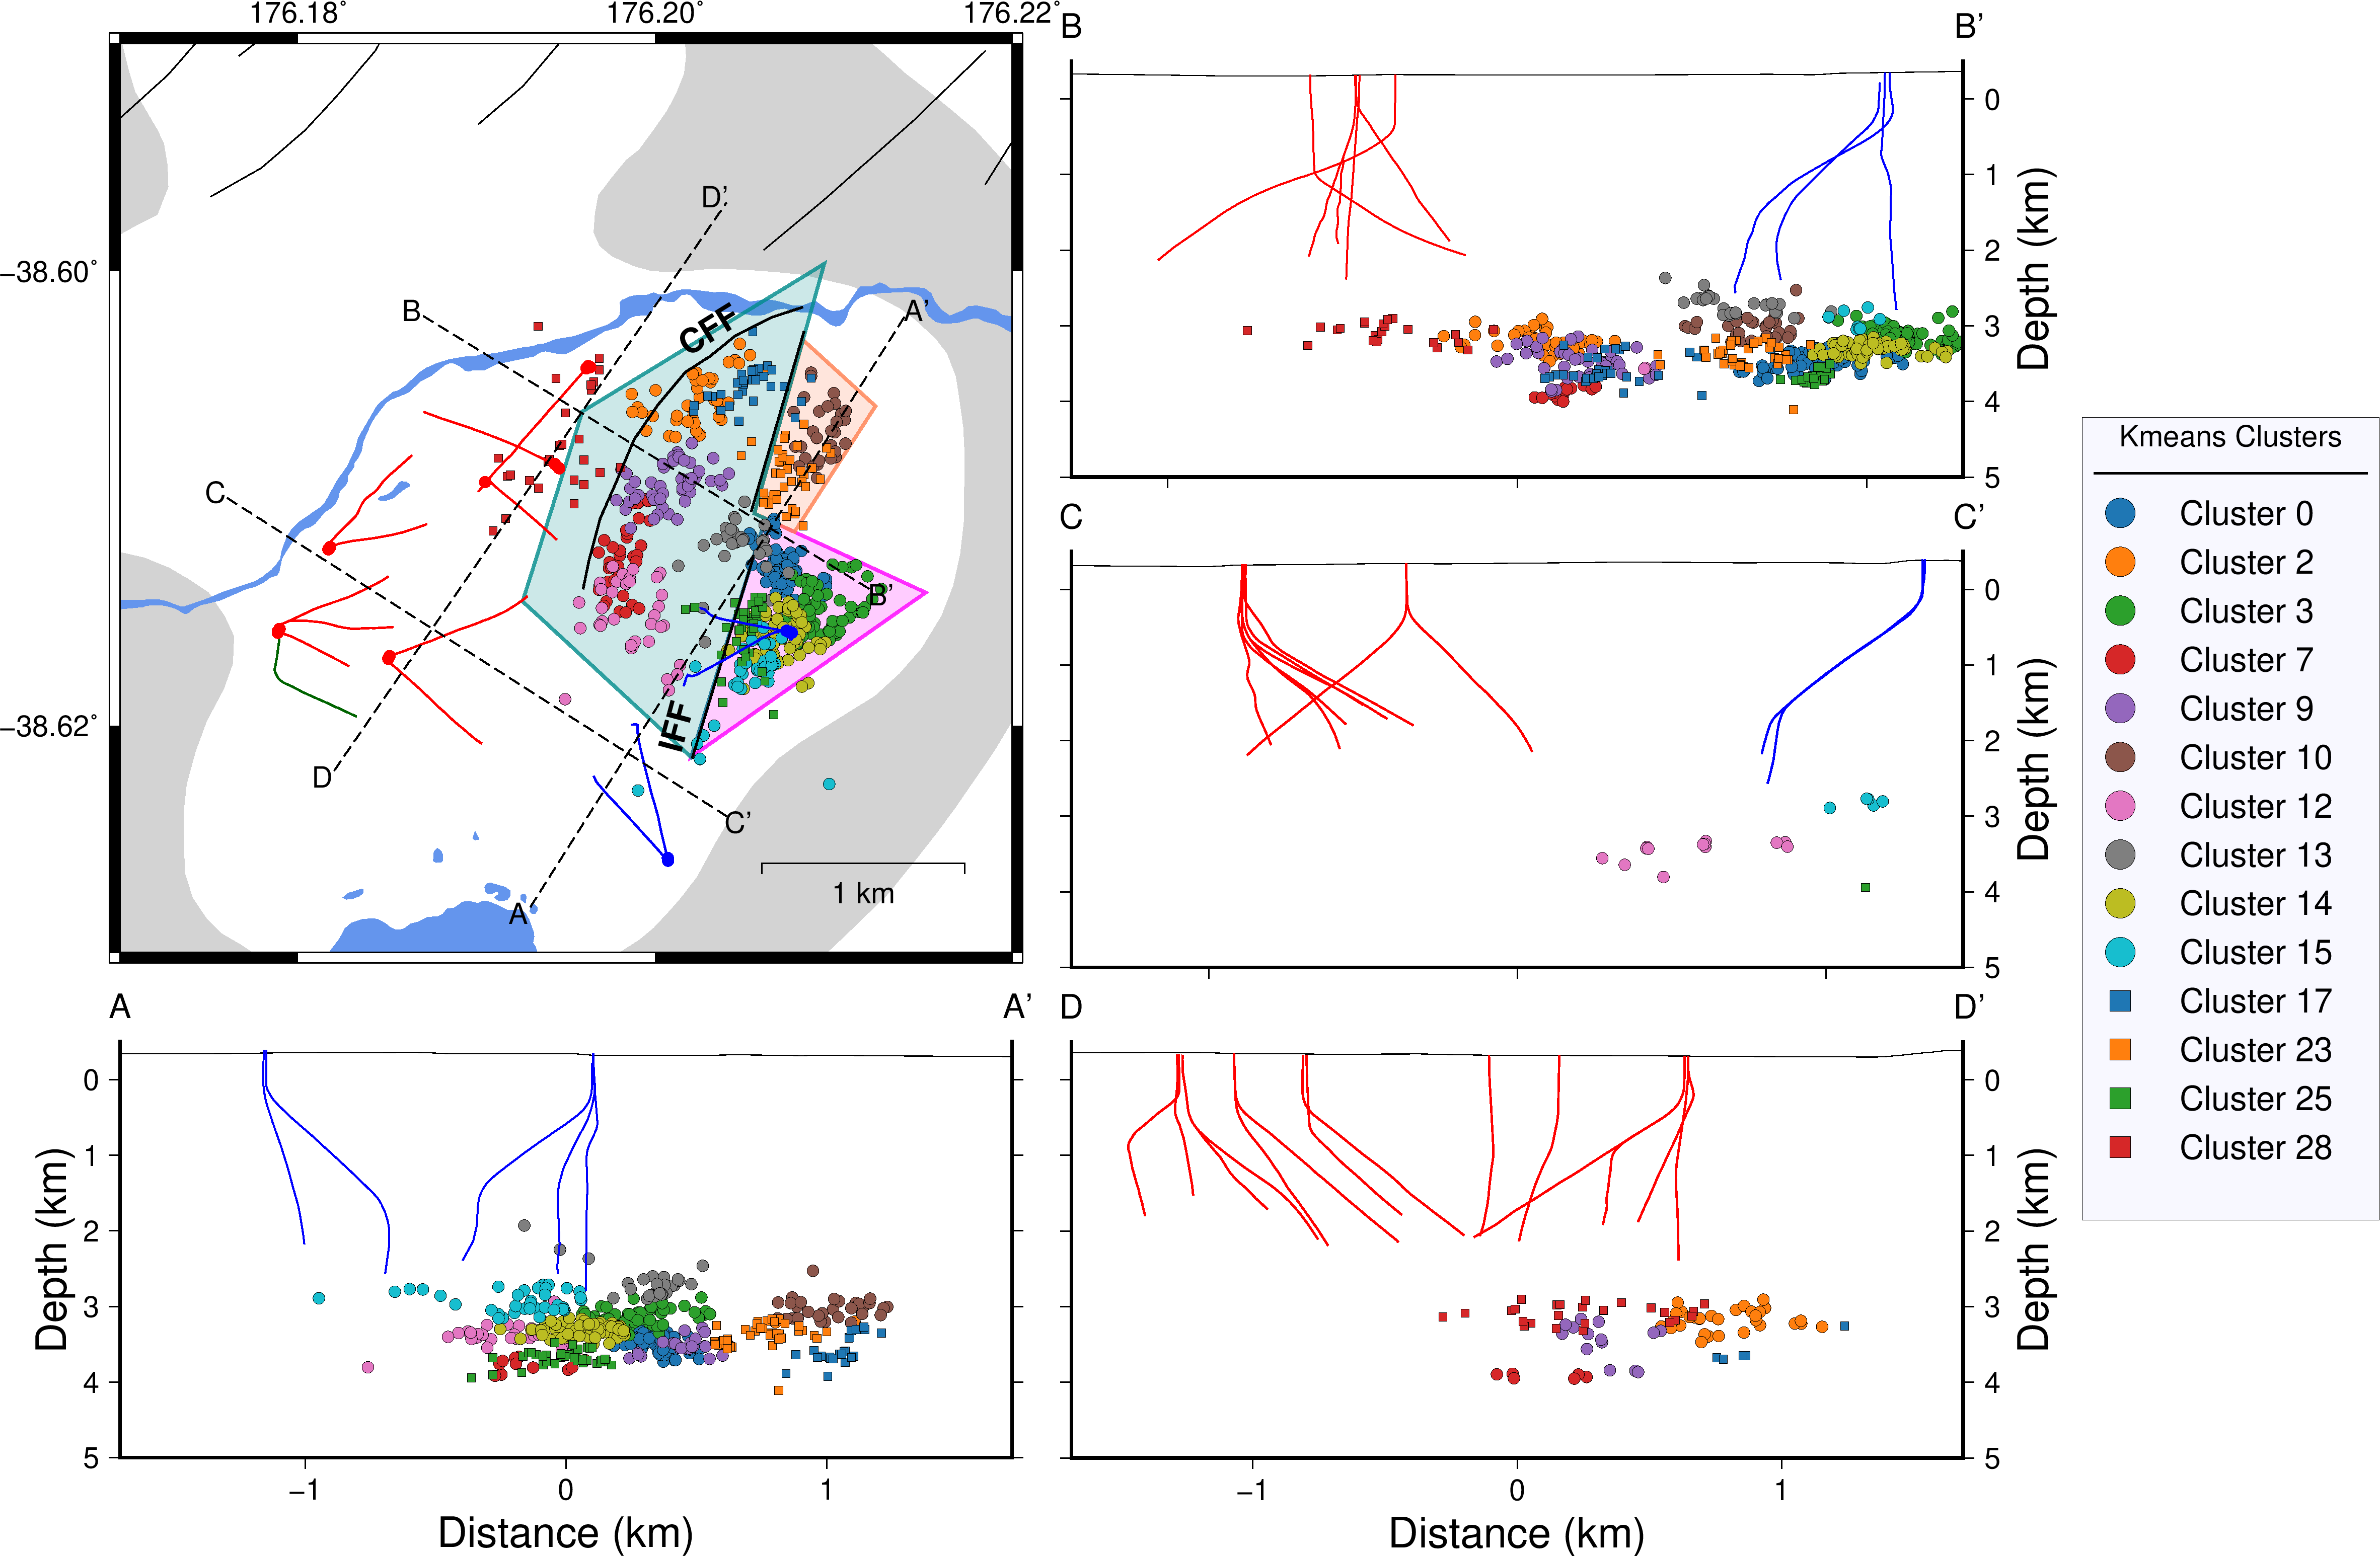
\includegraphics[width=0.75\textwidth,height=\textheight,keepaspectratio]{Chapter_5_FMs/figures/merc_Rot_GC_dets_kmeans_30/merc_Rot_kmeans_dets_30_comps}
\caption[Rotokawa kmeans clusters]{{
Rotokawa kmeans clusters ($k$=30) with greater than 20 events. Red and blue lines represent production and injection wells, respectively. The gray shaded area shows the resistivity boundary for the field \citep{Risk_2000} and black lines indicate active faults \citep{AFDB}. The colored polygons show the boundaries for the three inferred `compartments' defined in Chapter 4 based on linear features revealed in by earthquake hypocenters. The western compartment is green, southeastern pink and northeastern coral. These colors are used to map the polygons shown here in map view to the results presented in Figures \ref{434168} and \ref{237918}. 
{\label{878143}}%
}}
\end{center}
\end{sidewaysfigure}\selectlanguage{english}

Figure \ref{434168} shows the stress inversion results for each cluster, divided by compartment and color coded to match Figure \ref{878143}. From a first glance, it is clear that each inversion shows a normal faulting regime, with $\sigma_{1}\approx{\sigma_{V}}$. Only minor variations in the plunge of $\sigma_{1}$ are observed, but these are within the bounds of focal mechanism uncertainties ($\sim$30\textdegree{} angular deviation of the P axis).

Figure \ref{434168} also shows stress inversions that include all focal mechanisms in each compartment (white background, labeled `ALL'). In the western compartment, S$_{Hmax}$ is oriented 056\textdegree{} while in the northeast compartment, S$_{Hmax}$ is oriented 053\textdegree{}. For both of these compartments, $\nu$ approaches 1. In the southeast compartment, S$_{Hmax}$ is oriented 021\textdegree{} with a $\nu$ of 0.65. It is important to note that as the values of $\nu$ approach 1.0 throughout most of the reservoir, uncertainty in S$_{Hmax}$ also increases due to the ambiguity in the orientations of $\sigma_{2}$ and $\sigma_{3}$.

% Rotokawa kmeans inversions fig
\begin{sidewaysfigure}[p]
\begin{center}
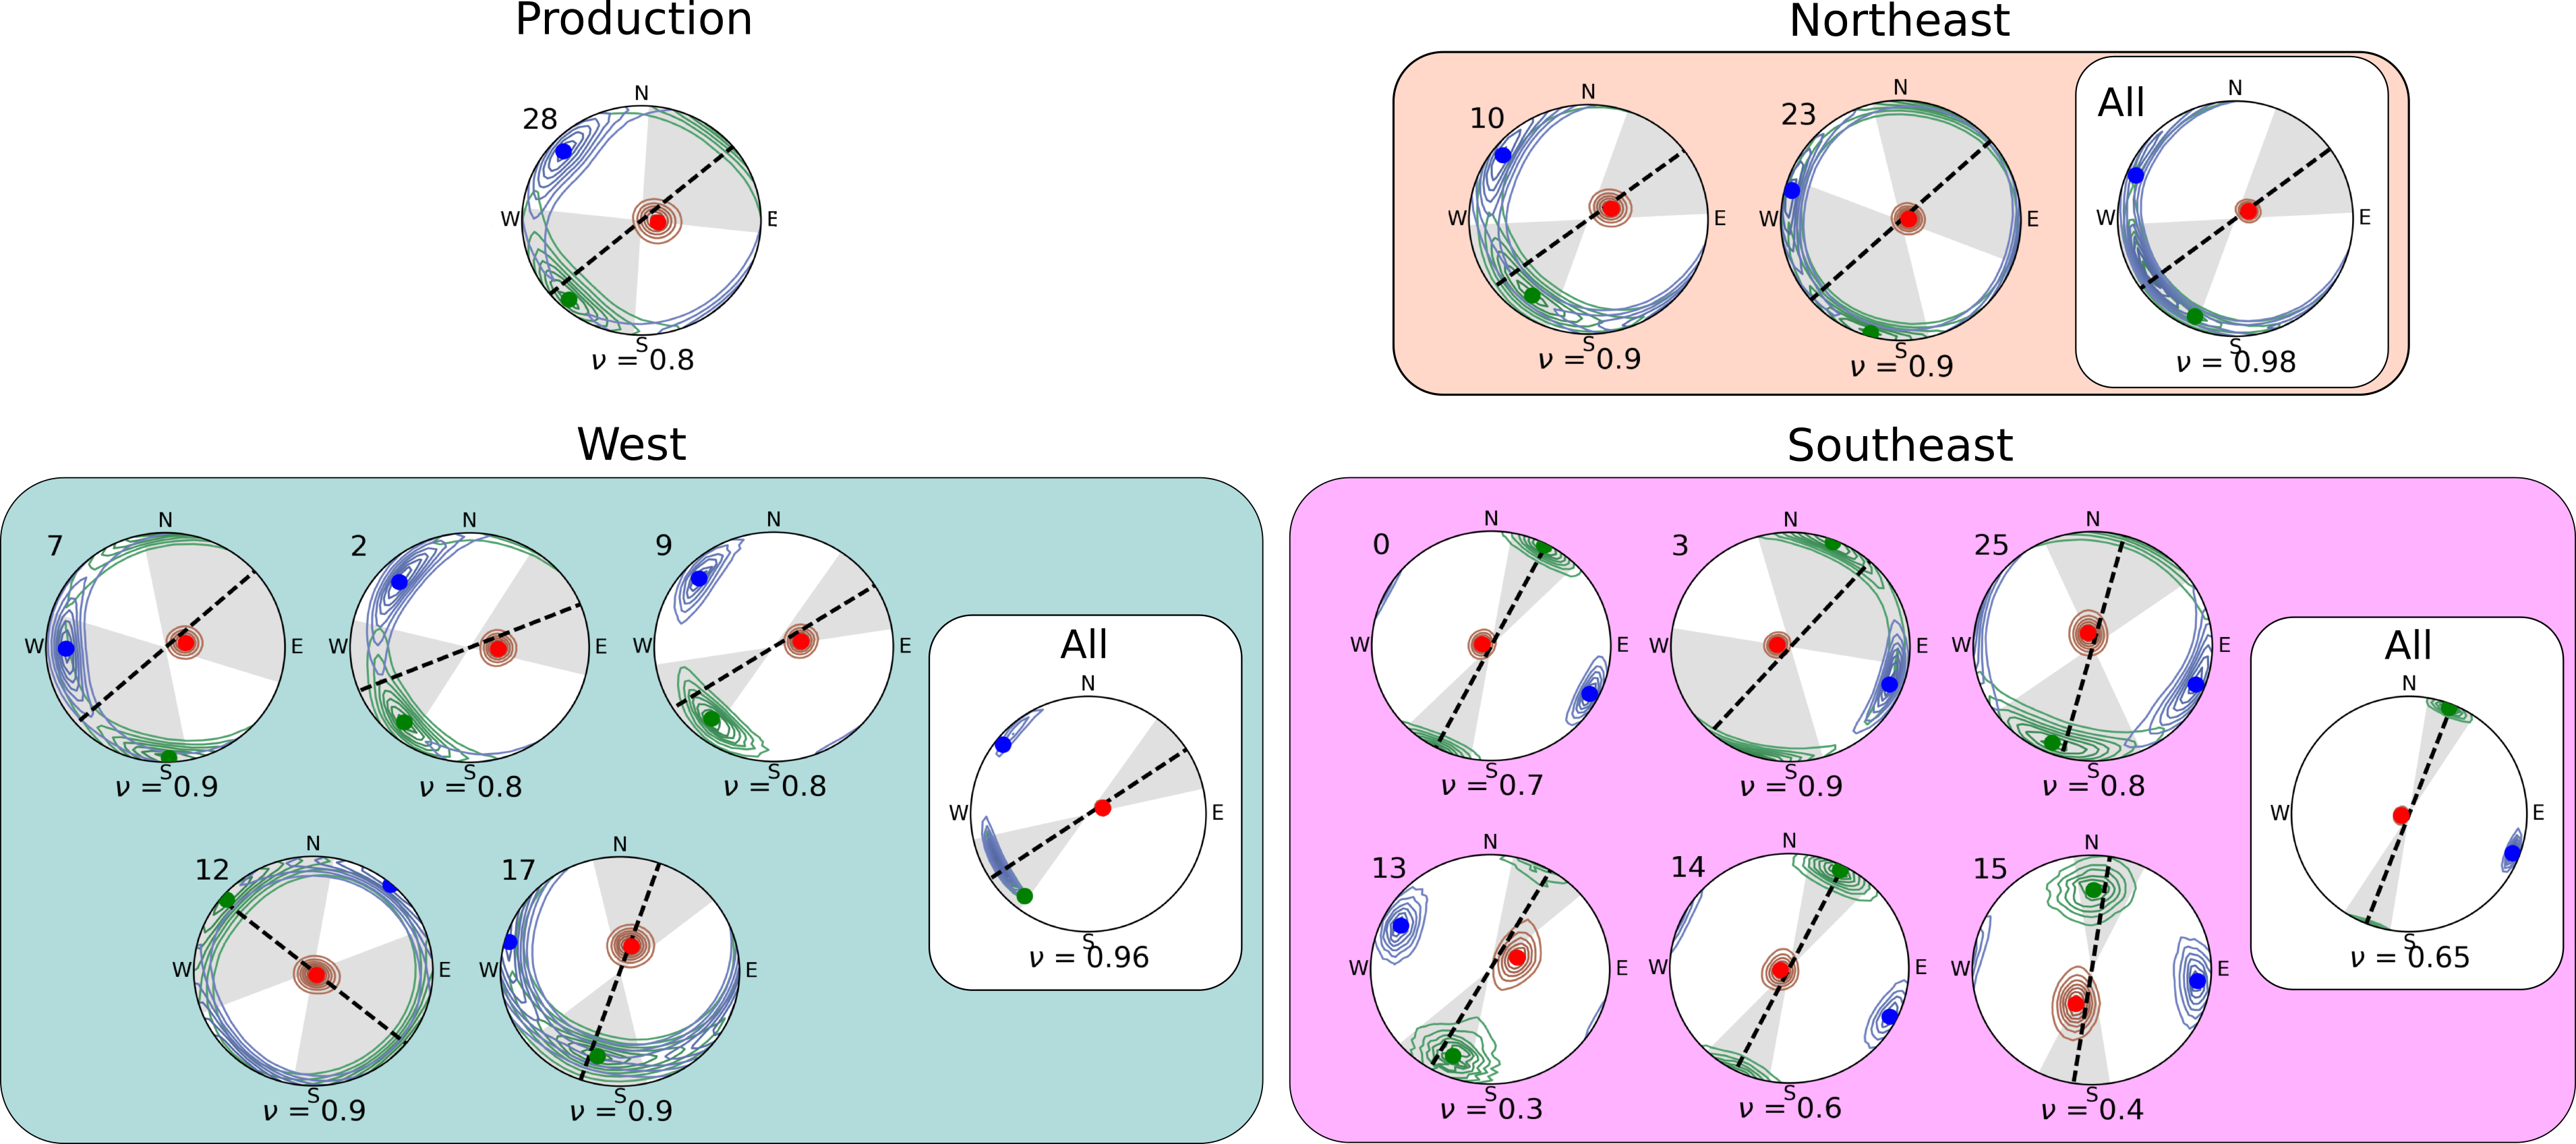
\includegraphics[width=\textwidth,height=\textheight,keepaspectratio]{Chapter_5_FMs/figures/Rot_kmeans_inversion_30/Rot_temps_GC_dets_kmeans_30_compartments_combined_lores}
\caption[Rotokawa stress inversions from kmeans clusters]{{
Lower hemisphere stereonets representing the stress inversion results for each k-means cluster shown in Figure~{\ref{878143}}. Red corresponds to $\sigma_{1}$, green to $\sigma_{2}$ and blue to $\sigma_{3}$, where the filled circle represents the maximum likelihood axis and the contours represent the shape of the PDF for that axis. The black dotted line shows the direction of maximum horzontal compressive stress (S$_{Hmax}$) for which the gray shaded bowtie shows the 90\% confidence region. Each plot is annotated below with the calculated stress ratio, $\nu$. Stereonets are grouped into three colored boxes indicating the compartment in which they are located. These boxes are color coded to match the compartment boundaries in Figure \ref{878143}. The stress inversion results using all focal mechanisms in each compartment are the solutions with the white background to the right of each box (labelled `ALL').
{\label{434168}}%
}}
\end{center}
\end{sidewaysfigure}\selectlanguage{english}

% Discussion
\section{Discussion}
\subsection{Ngatamariki}
\subsubsection{Stress inversion}\label{nga_stress_results}
The relatively small number of focal mechanisms calculated for Ngatamariki (205) precludes the extensive clustering that would allow us to analyze temporal variations in the stress state at the reservoir, as has been done elsewhere \citep[e.g.][]{Mart_nez_Garz_n_2013}. The five clusters shown in Figures \ref{nga_kmeans} and \ref{838980} reveal spatial variations similar to those found by \citep{j2019}. As expected, the three clusters in the southern injection field show a normal faulting regime with NE-SW S$_{Hmax}$, consistent with all previous studies of stress in the region \citep{hurst2002earthquake,hurst2008characteristics,Townend_2012}. The stress ratio, $\nu$, in Cluster 1, closest to the main injection well, NM06, is lower than in Clusters 4 or 9 (0.3 as compared to 0.4), but the uncertainties overlap considerably, and we therefore will not comment on their significance.

In the Ngatamariki northern injection zone, both Cluster 2 and 6 indicate a strongly deviated stress regime with no vertical principle stress. Between the two clusters, both $\nu$ and S$_{Hmax}$ vary considerably. S$_{Hmax}$ is 022\textdegree{} and 066\textdegree{} at Clusters 2 and 6, respectively, while $\nu$ is 0.8 and 0.1. The striking contrast between these two clusters, with cluster centroids located \textless{1} km apart, is puzzling. \citet{j2019} suggest that the tonalite intrusive body, encountered in both well NM08 and NM09, may be responsible for the deviation of the northern Ngatamariki stress state from an expected normal regime. The geometry and orientation of this intrusive is poorly constrained, with cutting found in only three wells \citep{Chambefort_2014}, making it difficult to assess its effect on stress locally. Unless it is highly irregularly shaped (e.g. a series of dikes/sills) we envision the intrusive having a similar effect on the stress state at both Cluster 2 and 6, which are located at similar depths and similar distances to the top of the intrusive. However, stress variations due to irregularities in the shape and orientation of the intrusive body (or bodies) provide the simplest explanation for the change in stress between the two clusters.

We foresee two other possible explanations for the contrast between Clusters 2 and 6 that are related to elevated pore-fluid pressure and\slash{or} reservoir cooling caused by fluid injection. The events belonging to Cluster 2 are likely related to injection into the nearest well, NM08, while those in Cluster 6 are located at the position of the \glspl{feedzone} of NM09. It is possible that differences in the injection parameters at NM08 and NM09 could explain the stress variation. However, as shown in Figure \ref{clust26}, \glspl{WHP_g} at both wells are modest during our study period (\textless{2} MPa). As pore-pressure acts equally on each of the principle stress components, such large deviations in $\nu$ and S$_{Hmax}$ are unlikely to be pore-pressure related. 

\begin{figure}[h!]
\begin{center}
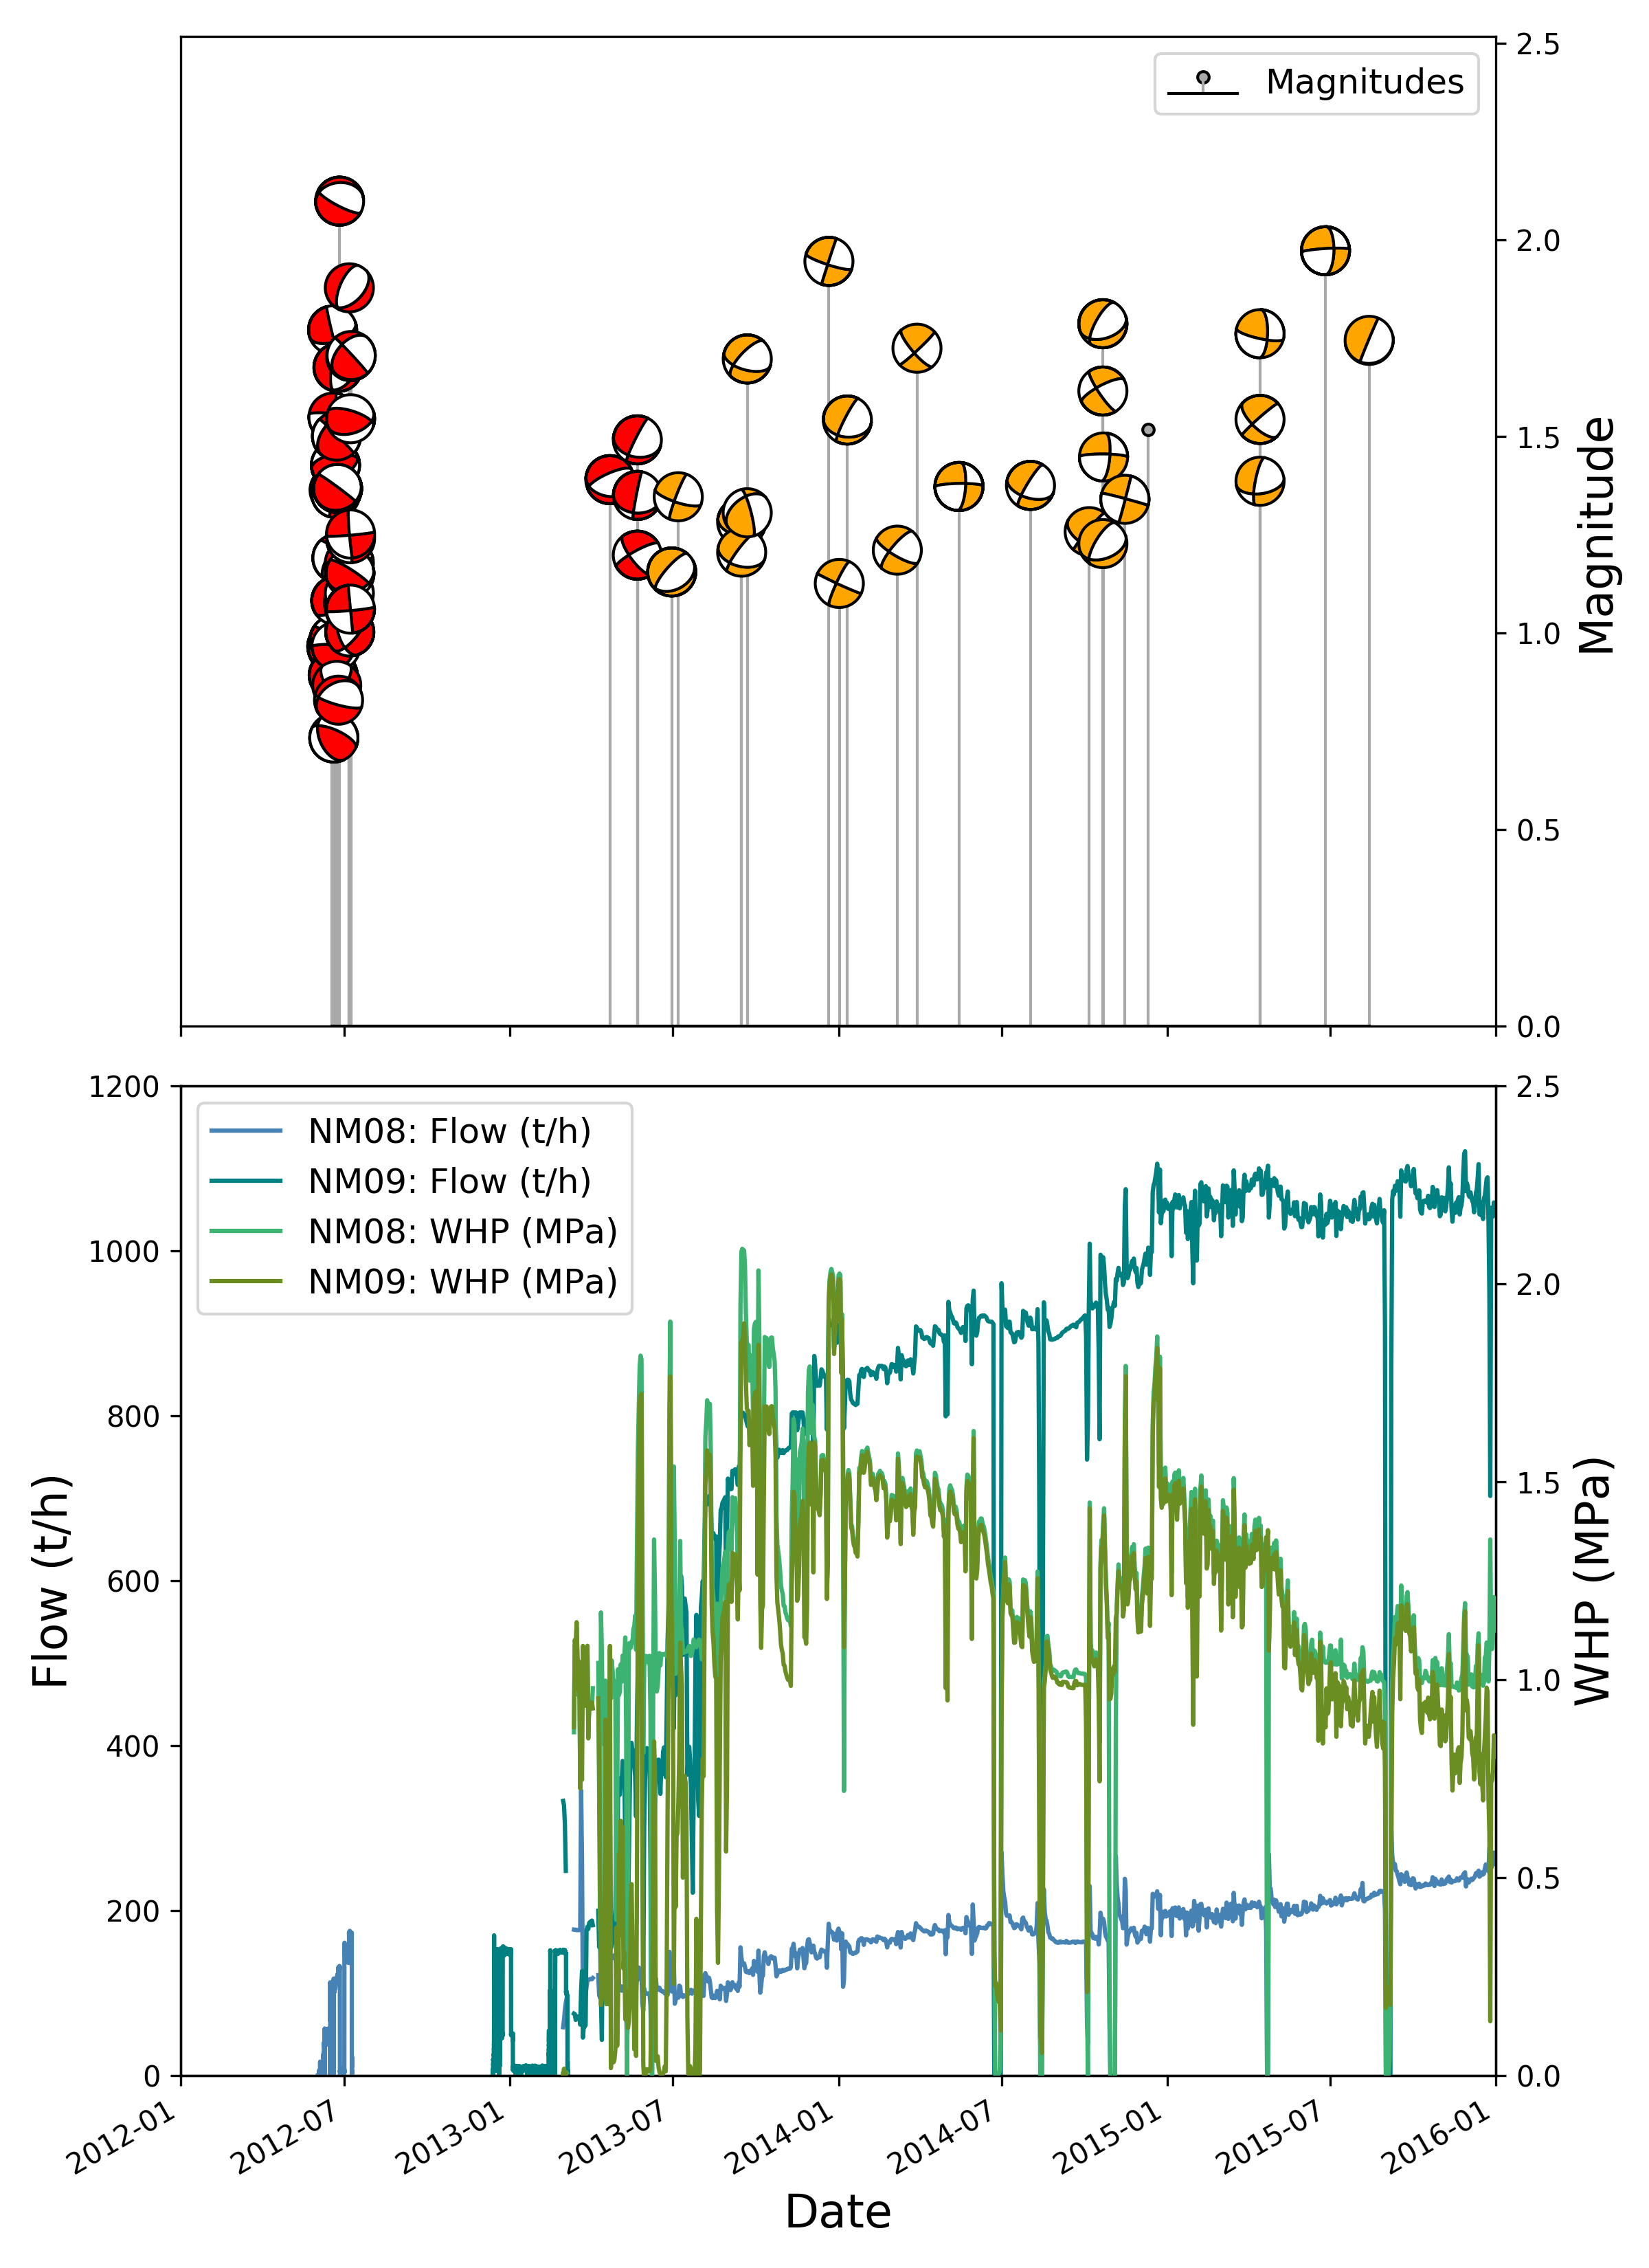
\includegraphics[width=0.84\columnwidth]{Chapter_5_FMs/figures/clust_2-6_comparison/NgaN_ALL_kmeans10_clusters_flow}
\caption[Ngatamariki Clusters 2 and 6 relative to injection flow rate]{{
Northern Ngatamariki \glspl{flow_rate}, \glspl{WHP_g}, and focal mechanisms. Cluster 2 (red) and Cluster 6 (orange) are shown as stems with the plan view lower-hemisphere focal mechanism solution as a head and the height corresponding to the magnitude of the event. Although the clusters were created via kmeans clustering based on euclidian distance between events, the clusters are also perfectly split in time with Cluster 2 occurring early in the study period, and Cluster 6 occurring later.
{\label{clust26}}%
}}
\end{center}
\end{figure}

As mentioned in Section \ref{stress_background}, thermoelastic stress reduction near injection wells can produce large deviations in the local stress state \citep{Jeanne_2015tensor}. While the simplest explanation for the contrast in stress between Clusters 2 and 6 is related to the intrusive body, we believe that reservoir contraction due to cold water injection presents a compelling alternative explanation. The degree to which a reservoir with fracture-dominated \gls{permeability} contracts in response to cold water injection is related to a number of factors that describe both the reservoir (e.g. rock bulk modulus and fracture spacing) as well as the injection itself (injectate temperature and \gls{flow_rate}) \citep{stephens1982hydraulic}. Although the injectate temperature at both wells is similar, the rate of injection is not. NM08 is less permeable than NM09 and, as a result, accepts only $\sim$250 t/h as compared to the nearly 1100 t/h injected at NM09 (Figure \ref{clust26}) resulting in total injected volumes over our study period of 4.19e6 m$^3$ and 2.07e7 m$^3$, respectively. We would therefore expect the cooling-related stresses at NM09 to be more significant than at NM08.

However, it is worth emphasizing that the majority of events in Cluster 2 occurred during the \gls{stimulation} of NM08 (duration of one month) and not over the entire study period (Figure \ref{clust26}). As these events occurred $\sim$200 m from the main \glspl{feedzone} at NM08, thermal \gls{diffusivity} (measured in mm$^2$/s \citep{Kanamori_1968}) and short duration of \gls{stimulation} make it unlikely that they were influenced by cooling from the well. In contrast, the events in Cluster 6 are well-distributed over a longer period and are therefore more likely to have been influenced by thermoelastic stresses. The extent of reservoir cooling has been confirmed by \acrshort{PTS} runs at monitoring well NM02 ($\sim$250 m from NM09), where temperatures at reservoir depths had cooled by $\sim$100\textdegree C within 3 years of the start of injection (Steve Sewell, personal comm.). Therefore, the cooling zone extending from NM09 likely encompasses most of the events in Cluster 6 and likely extends further towards the production field, although it has not yet reached well NM07 (Figure \ref{nga_kmeans}). We can be confident that the stress inversion of Cluster 6 is therefore affected by thermoelastic stresses.

If the cooled zone around NM09 is larger in the vertically than it is laterally (picture a pipe oriented vertically), it will have reduced $\sigma_{1}$ by more than $\sigma_{2}$ or $\sigma_{3}$. Such a scenario may help explain the lower stress ratio and different faulting regime observed in Cluster 6 when compared with Cluster 2. A similar phenomenon was observed and modeled by \citet{Jeanne_2015tensor,Mart_nez_Garz_n_2013} at The Geysers, where a normal faulting regime above and below the reservoir has become a strike-slip regime within it as a result of cooling at the injection wells.

\subsection{Rotokawa}
\subsubsection{Spatial stress variation}
As demonstrated in Figure \ref{434168}, deviations in stress state at Rotokawa are somewhat less dramatic than between northern and southern Ngatamariki. For each of the clusters at Rotokawa, $\sigma_{1}\approx{\sigma_{V}}$, with only minor variations in dip that cannot be confidently resolved. However, there are spatial variations in both S$_{Hmax}$ and $\nu$ that deserve further inspection. Specifically, values for S$_{Hmax}$ and $\nu$ in the southeast compartment, nearest the injection wells, are distinct to those in other parts of the field (Figure \ref{434168}).

Borehole measurements of drilling-induced tensile failure in the production field (RK18L2, RK32, RK30L1) \citep{McNamara_2015} show that S$_{Hmax}$ ranges from 025--049\textdegree{}. They also demonstrate that lateral stress changes in the reservoir are significant and can occur over distances of \textless{1} km. However, as no images were obtained from any of the current injection wells, we have little constraint on the orientation of stress or fractures in the seismically active part of the field. Inverting for the stress state using all mechanisms in the southeast compartment, S$_{Hmax}$ is 021\textdegree{} with a stress ratio, $\nu$, of 0.65. For all mechanisms in the western compartment, S$_{Hmax}$ is 056\textdegree{} and $\nu$ approaches 1, while in the northeast compartment S$_{Hmax}$ is 053\textdegree{} and $\nu$ also approaches 1. These values for S$_{Hmax}$ are roughly consistent with directions obtained from the borehole measurements \citep{McNamara_2015}.

In Figure \ref{533041} we show the stress inversion results projected onto the horizontal plane as bowties showing the 90\% confidence interval for S$_{Hmax}$, colored by the stress ratio. While it is tempting to interpret the apparent anticlockwise rotation of S$_{Hmax}$ in the southeast compartment (relative to the rest of the field) as related to injection well proximity, there are a number of caveats. Most importantly, stress ratios approaching 1.0 in the rest of the reservoir suggest that $\sigma_{2}$ and $\sigma_{3}$ have similar magnitudes. Given that $\sigma_{2}$ and $\sigma_{3}$ are horizontal here, stress inversion from focal mechanisms cannot adequately resolve the true direction of S$_{Hmax}$ for a stress ratio of 1. So while an azimuth of 021\textdegree{} for S$_{Hmax}$ in the southeast compartment is relatively well constrained, interpreting it in the context of S$_{Hmax}$ throughout the rest of the reservoir is unwarranted.

Although stress ratio is the least well-resolved parameter resulting from the inversion of focal mechanisms, we can at least say with some confidence that $\nu$ is lower, on average in the southeast compartment than in the rest of the reservoir. As the southeast compartment contains, or is adjacent to, injection wells RK20, 23 and 24, it is subject to some of the highest pore pressures and temperature gradients in the field. As discussed for Ngatamariki, it is difficult to envision a scenario in which elevated pore pressures of $\sim$1 MPa would deviate the in situ stress state in any discernible way, especially given that pore pressure affects each principle stress axis equally. A decrease of 1 MPa for all principle stress axes will change the stress ratio by some small amount, but this is unlikely to be measurable through focal mechanism inversion.

Instead, we believe the only injection-related process capable of producing significant stress changes at Rotokawa is the cooling of the reservoir host rock. As injection had been occurring in the current configuration (i.e. at wells RK20--24) for at least five years by the end of our study period, the cooling front would have had time to reach the boundaries of our inferred southeast compartment, and likely the southern portions of the western compartment as well. Numerical modeling of The Geysers geothermal field in California has shown that stress reductions measured in 10's of MPa are possible over time spans of 2--5 years for similar injectate temperatures and in situ stress state to what is encountered at Rotokawa \citep{Jeanne_2015tensor}. These stress changes are greatest directly adjacent to the wells, as would be expected, because there the fluid is coldest and the induced thermal gradient is the greatest. As the cool, denser fluid enters the reservoir, it flows downward, driven by gravity. This gravity flow results in a vertically elongate zone of cooling, which preferentially reduced whichever stress axis is most vertical \citep{Jeanne_2015tensor}. In the case of The Geysers, Rotokawa and Ngatamariki, this means preferential reduction of $\sigma_{1}$, which has the effect of limiting the population of fractures oriented for failure and reducing the stress ratio. As the injected fluid begins to heat and flow laterally, the zone of cooling also elongates in the direction of greatest lateral \gls{permeability}, likely subparallel to S$_{Hmax}$, along strike of structures such as the \acrshort{IFF} or \acrshort{CFF}, which are well oriented for failure in the regional stress regime. We envision a complex interplay between the state of stress and the geometry of the zone of cooling at Rotokawa, where faults that are well-oriented for failure also define a preferred axis of cooling. It is possible that preferential reduction of $\sigma_{1}$ due to gravity-driven flow in the southeastern compartment has led to a reduced stress ratio in this portion of the field and that a limited degree of cooling further from the wells has left the stress state largely unchanged.

% Rotokawa SHmax figure
\begin{figure}[h!]
\begin{center}
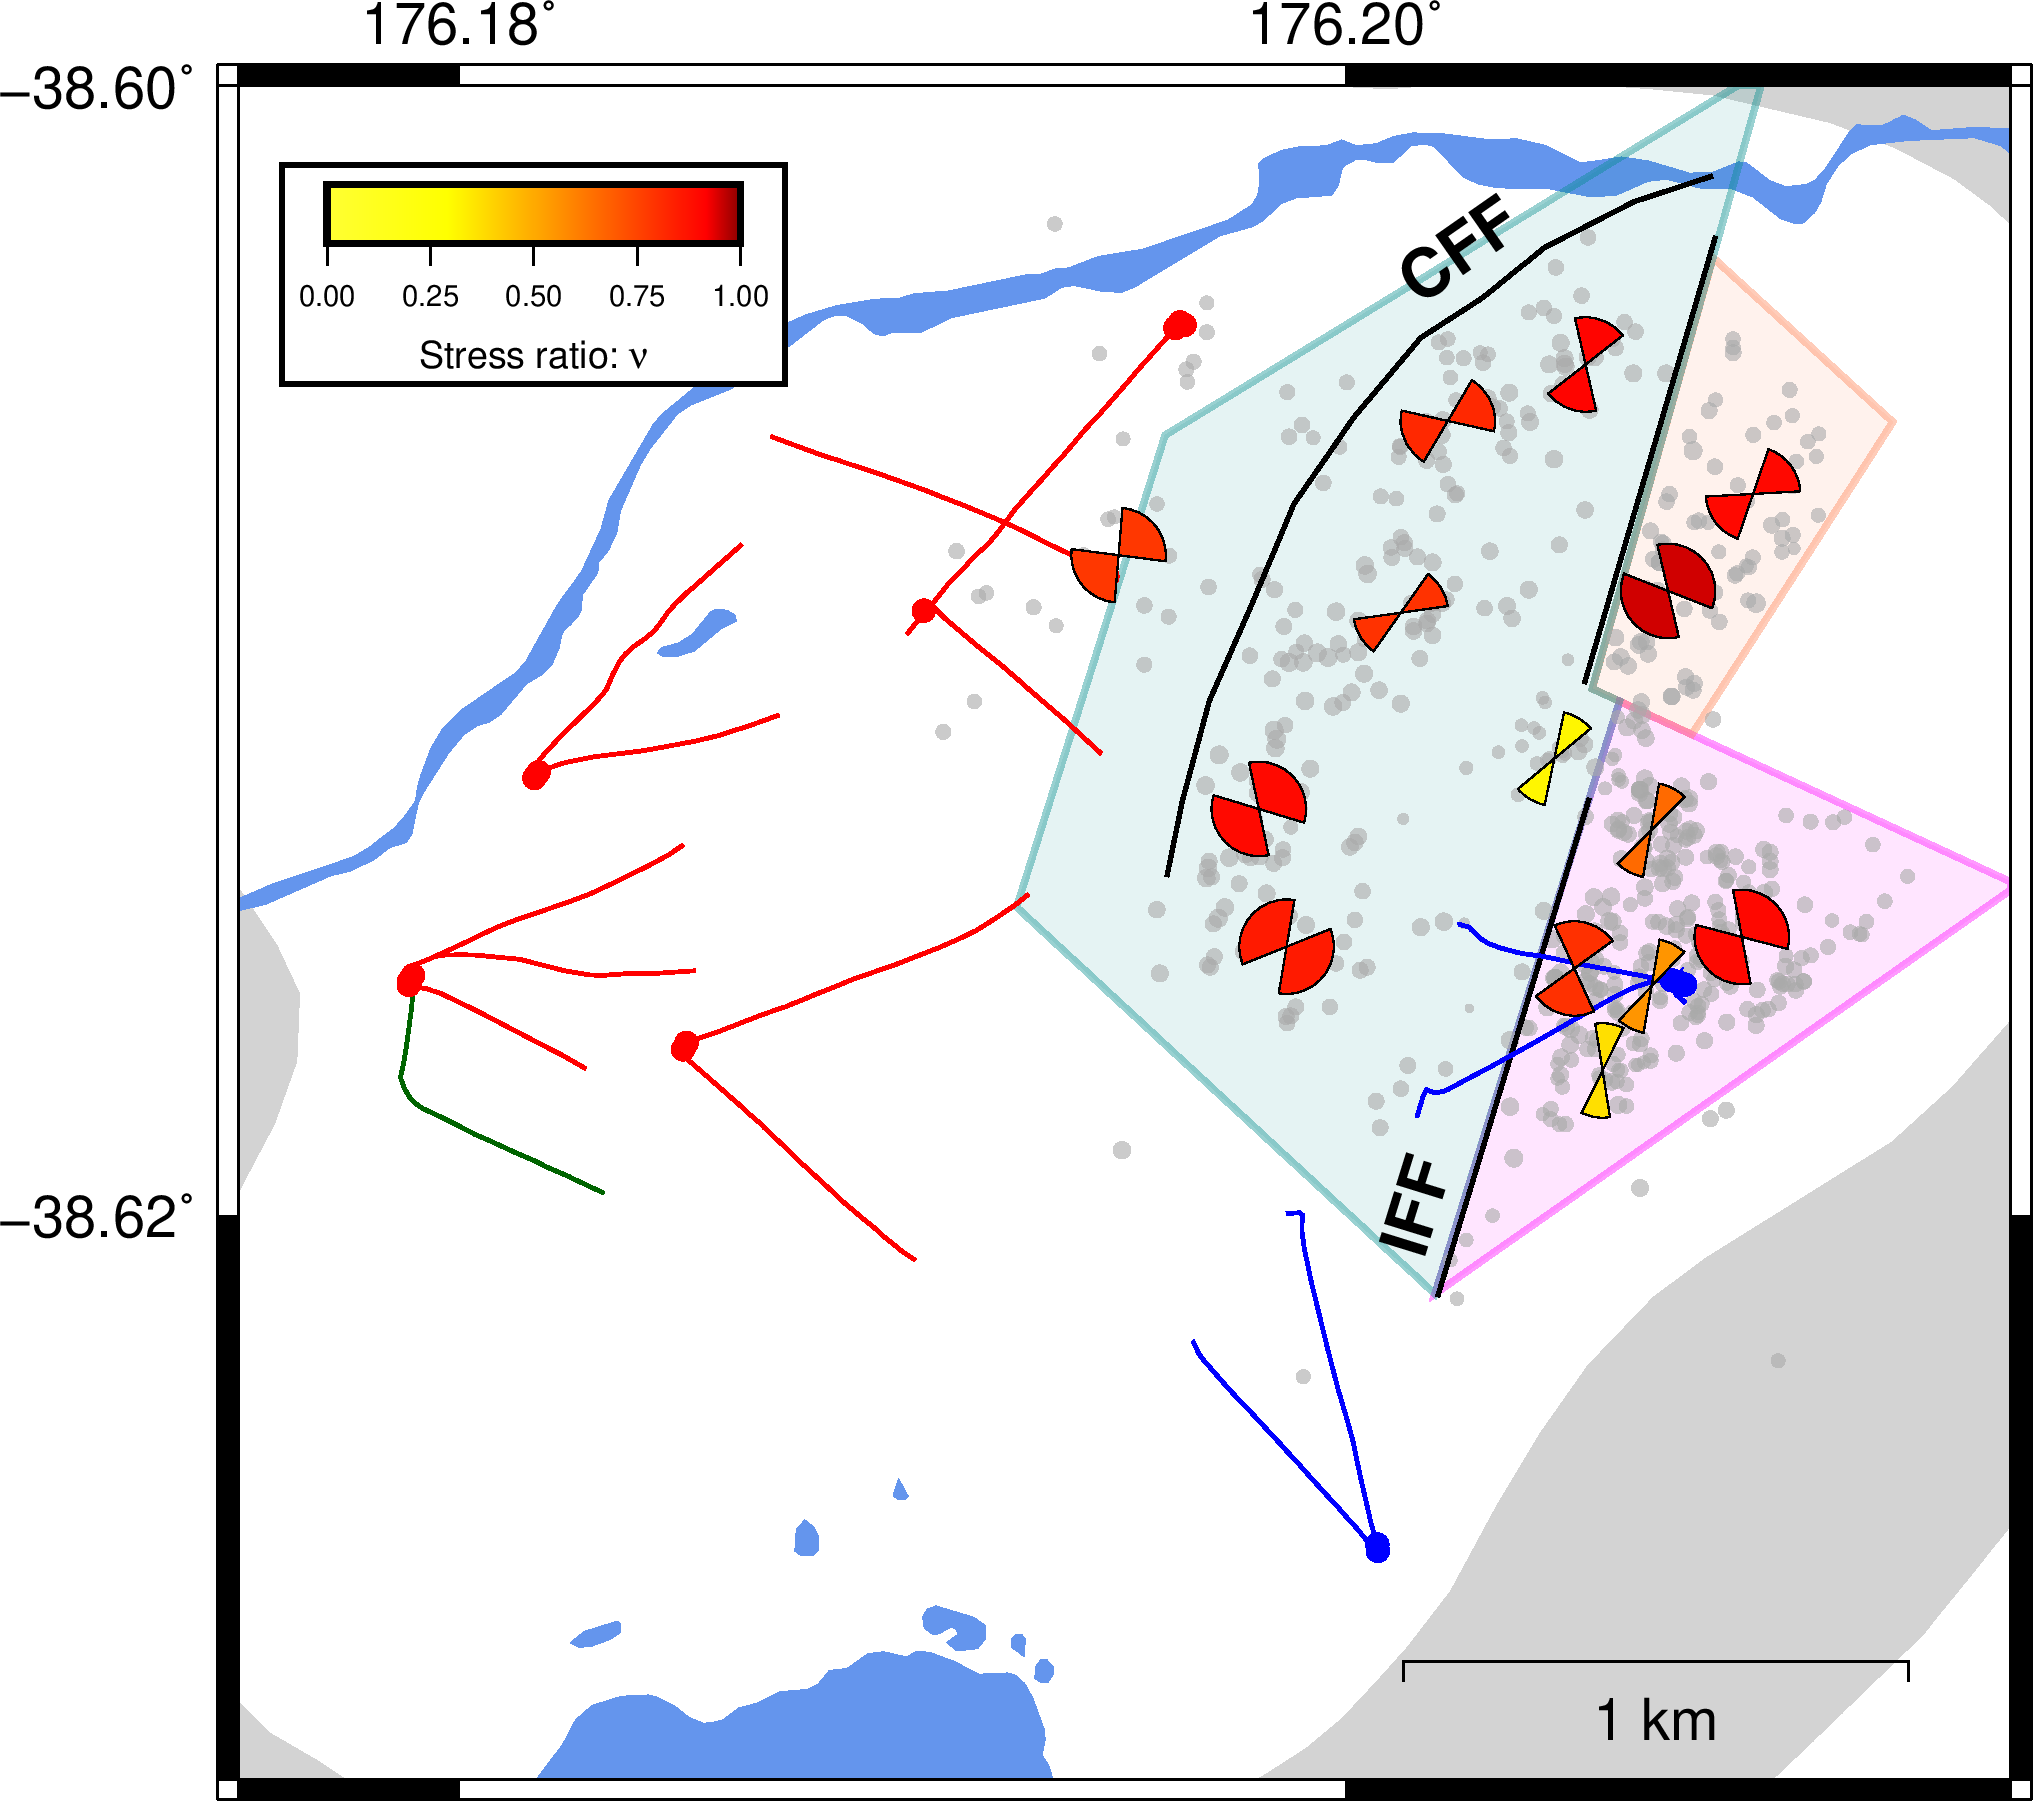
\includegraphics[width=0.84\columnwidth]{Chapter_5_FMs/figures/merc_Rot_kmeans_cents_40_sigmas_seis_nu/merc_Rot_dets_kmeans_30_cents_SHmax_nu_comps}
\caption[S$_{Hmax}$ and $\nu$ for kmeans clusters at Rotokawa]{{
S$_{HMAX}$ directions for the kmeans clusters (Figure \ref{878143}) at Rotokawa. Bowties show the 90\% confidence intervals for S$_{Hmax}$, colored by the stress ratio, $\nu$.
{\label{533041}}%
}}
\end{center}
\end{figure}


\subsubsection{Temporal stress variation}
Finally, we compare stress parameters from focal mechanism inversion to temporal changes in injection at Rotokawa. Due to the vertical $\sigma_{1}$ and high stress ratio in the western and northeastern compartments, S$_{Hmax}$ is poorly constrained and we therefore avoid further subdividing these areas for temporal analysis. In the southeast compartment, the calculated stress ratio is lower than elsewhere in the field and S$_{Hmax}$ is better constrained. Its proximity to injection wells means that this compartment is also the most likely to show signs of injection-induced stress change. We therefore divide the 304 focal mechanisms in this compartment into time-sequential groups of 55 events, and invert for the stress states in each group, advancing the inversion by steps of 10 events between data points. As $\sigma_{1}\approx{\sigma_{V}}$ for all clusters at Rotokawa, we plot S$_{Hmax}$ and $\nu$ with time versus the injection rates from RK20, 23 and 24 (Figure \ref{IFF_temporal}). 

\begin{figure}[h!]
\begin{center}
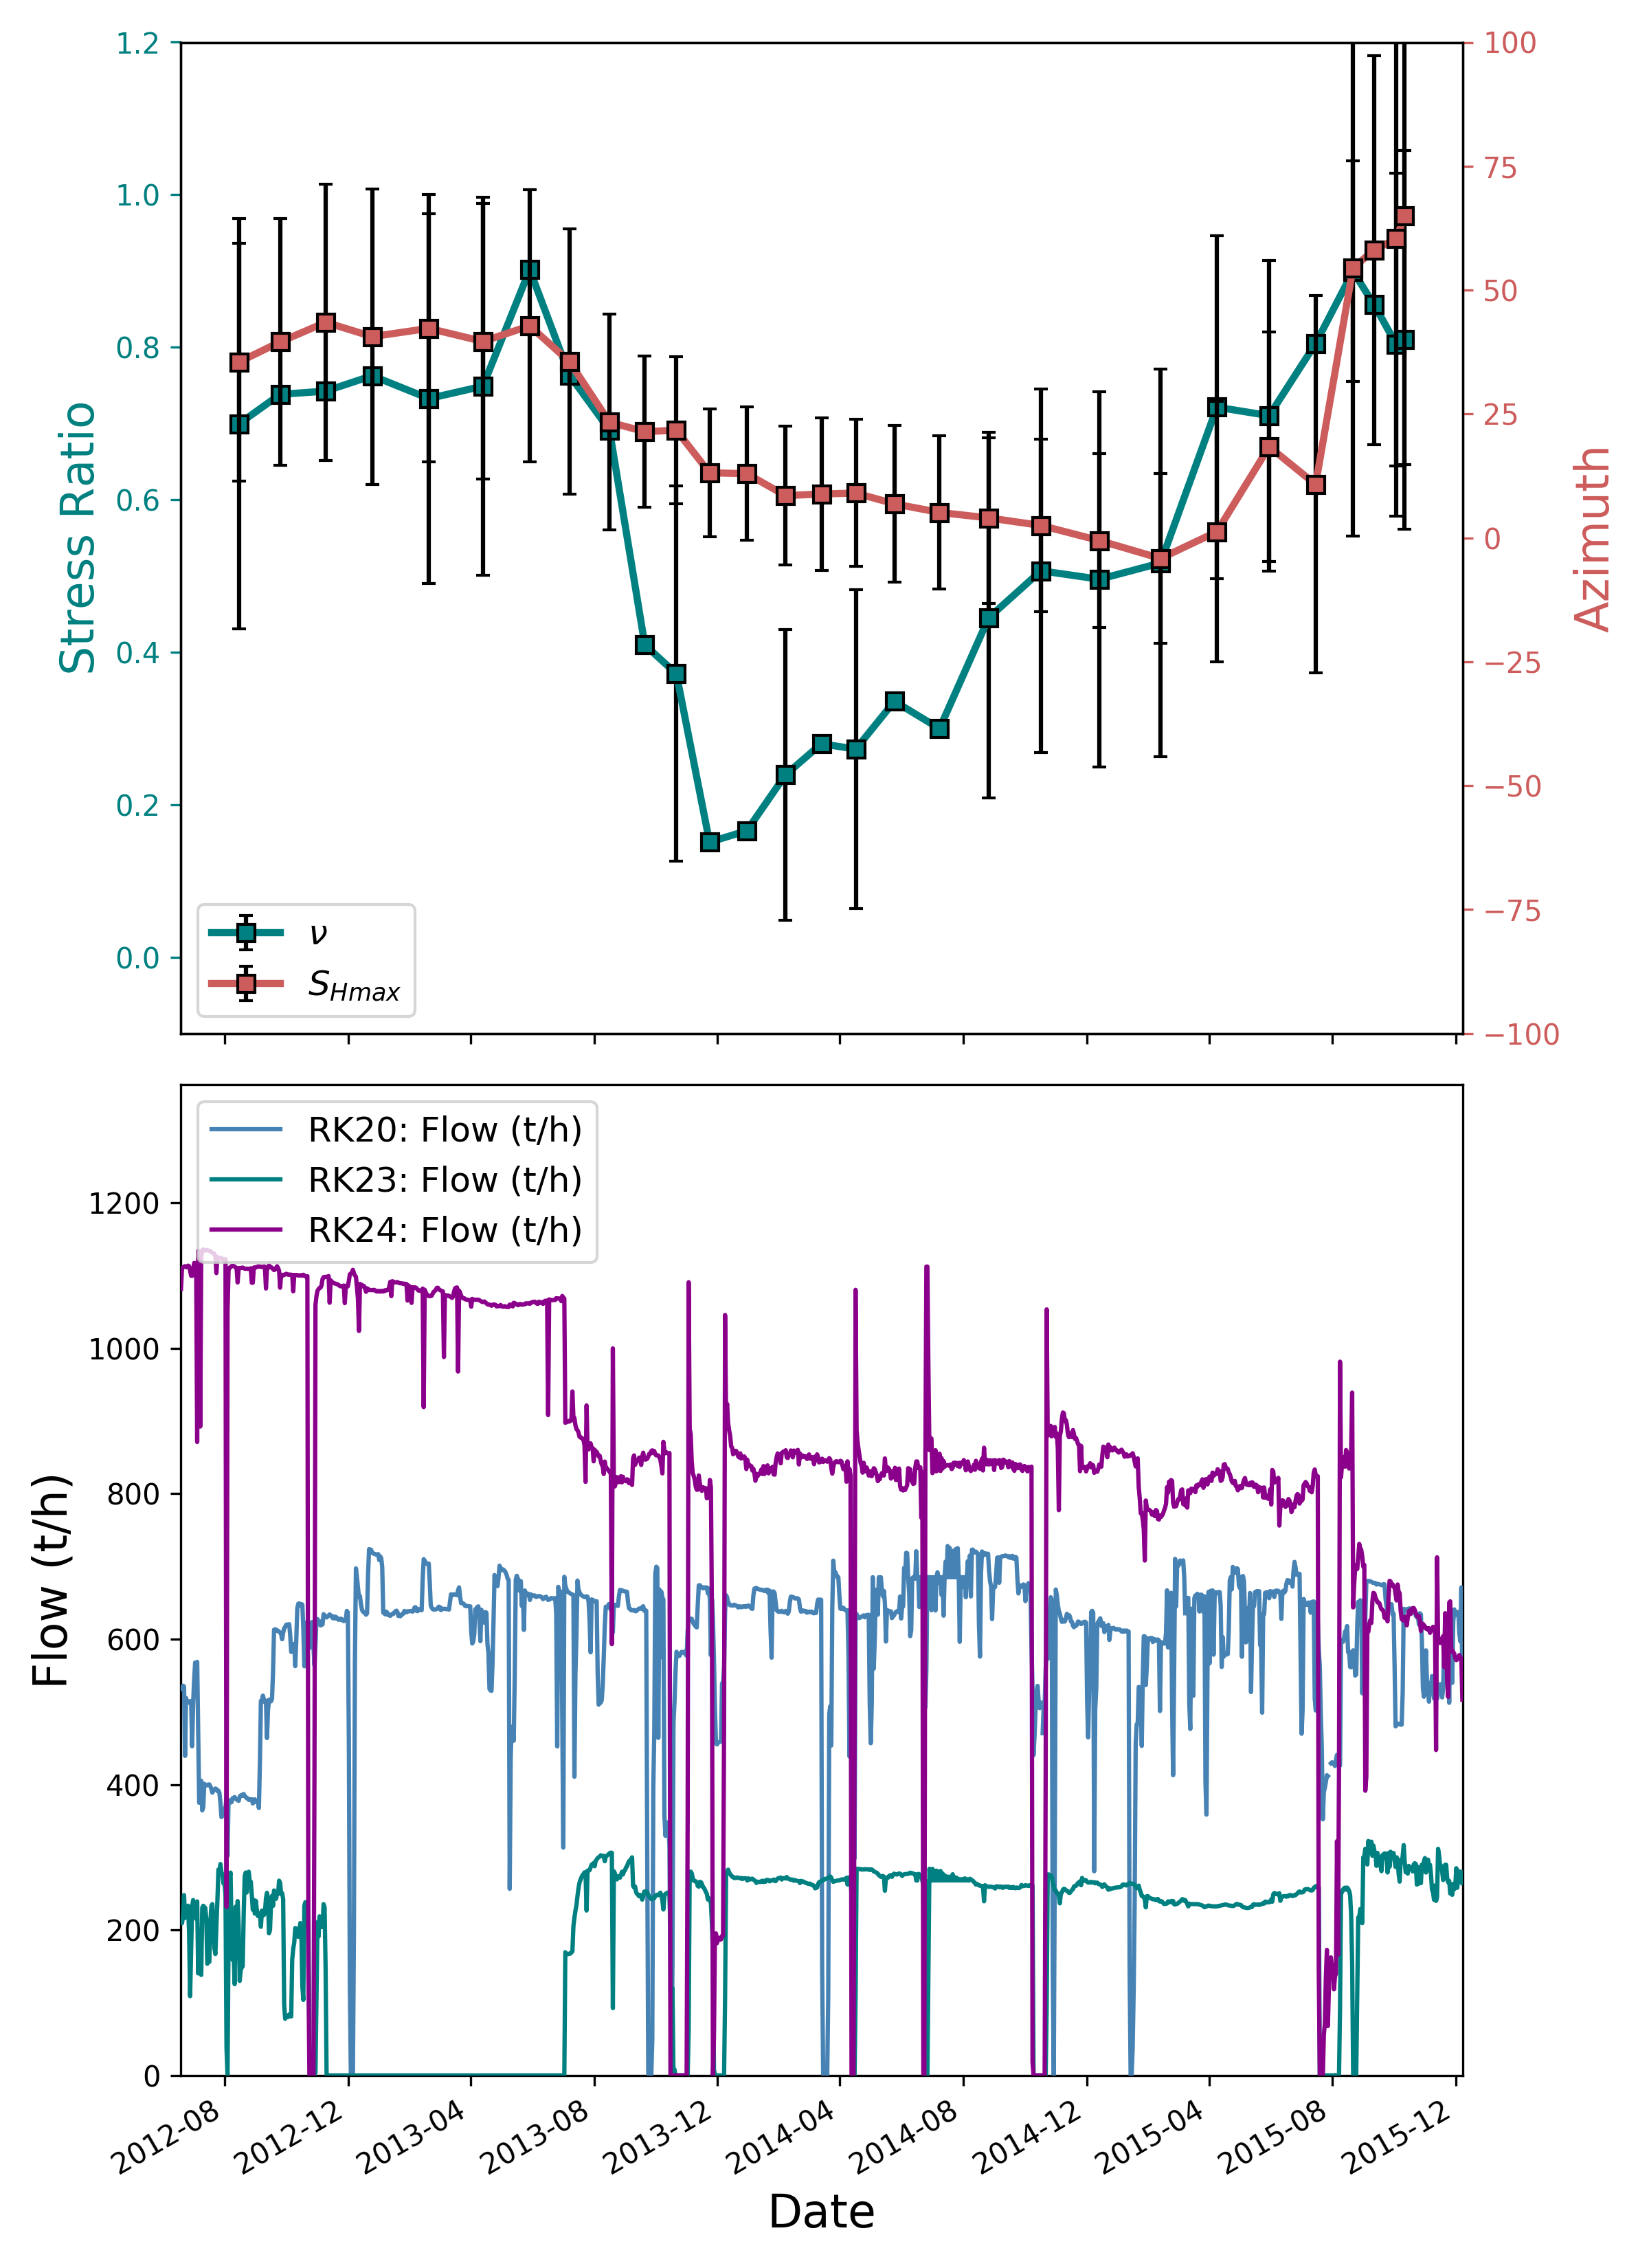
\includegraphics[width=0.84\columnwidth]{Chapter_5_FMs/figures/Rot_IFF_temporal/IFF_wedge_nu_Shmax_w_time_win55_ol45_RK20-23-24}
\caption[S$_{Hmax}$ and $\nu$ with time near injection wells at Rotokawa]{{
Stress inversions in the southeastern compartment at Rotokawa with time. Each data point corresponds to a cluster of 55 consecutive focal mechanisms with an overlap of 45 events between adjacent data points. Points are plotted at the time average for each subset of events. The lower panel shows \glspl{flow_rate} for injection wells RK20, 23 and 24 during the study period.
{\label{IFF_temporal}}%
}}
\end{center}
\end{figure}

Both S$_{Hmax}$ and $\nu$ appear to respond to the injection changes at wells RK23-24 during the last half of 2013. $\nu$, in particular, decreases from near 1.0 to below 0.2 over the six months following the injection shift from RK24 to RK23. If our interpretation of the orientation of the \acrlong{IFF} is correct, and it also serves as a barrier to cross strike flow, then the stress state to the east of the \acrshort{IFF} would respond most strongly to RK23, which is the only well on the eastern side of the fault. If this is the case, then the decrease in $\nu$ and anticlockwise rotation of S$_{Hmax}$ shown in Figure \ref{IFF_temporal} may correspond to the restart in injection at RK23 after $\sim$8 months of inactivity. As described in Section \ref{nga_stress_results}, such a decrease in $\nu$ could reflect preferential cooling of $\sigma_{1}$ (Figure \ref{cooling}). This makes sense in the context of a well that has been inactive for a number of months. During this time, the near-well reservoir would have had ample time to re-heat to near the natural state temperature. Once injection restarted (Figure \ref{cooling}a), the temperature contrast would have encouraged gravity-driven, downward flow from the well and a corresponding decrease in $\nu$. Interestingly, $\sim$7 months after the restart of injection at RK23, $\nu$ began to rebound, eventually returning to elevated levels (\textgreater{0.8}) by the end of the study period. The steep drop and more gradual rebound of $\nu$ may tell us something about the time scale and geometry of reservoir cooling. If a decrease in $\sigma_{1}$ corresponds to the drop in $\nu$ due to downward flow, perhaps the rebound in $\nu$ reflects a transition from downward to lateral flow (Figure \ref{cooling}b), likely along fractures subparallel to $\sigma_{2}$ (S$_{Hmax}$). As flow transitions from gravity-driven to lateral, the shape of the cooled zone of the reservoir changes from a sub-vertical cone beneath the well to one with a larger lateral footprint. If lateral \gls{permeability} is anisotropic, favoring flow in the direction of S$_{Hmax}$, as we would expect, then the zone of cooling would also be elongate in this direction, thereby cooling S$_{Hmax}$ more than $\sigma_{3}$ (Figure \ref{cooling}b). Such a scenario could produce an increase in $\nu$ similar to what we observe in the southeast compartment at Rotokawa.

% cooling schematic
\begin{sidewaysfigure}[p]
\begin{center}
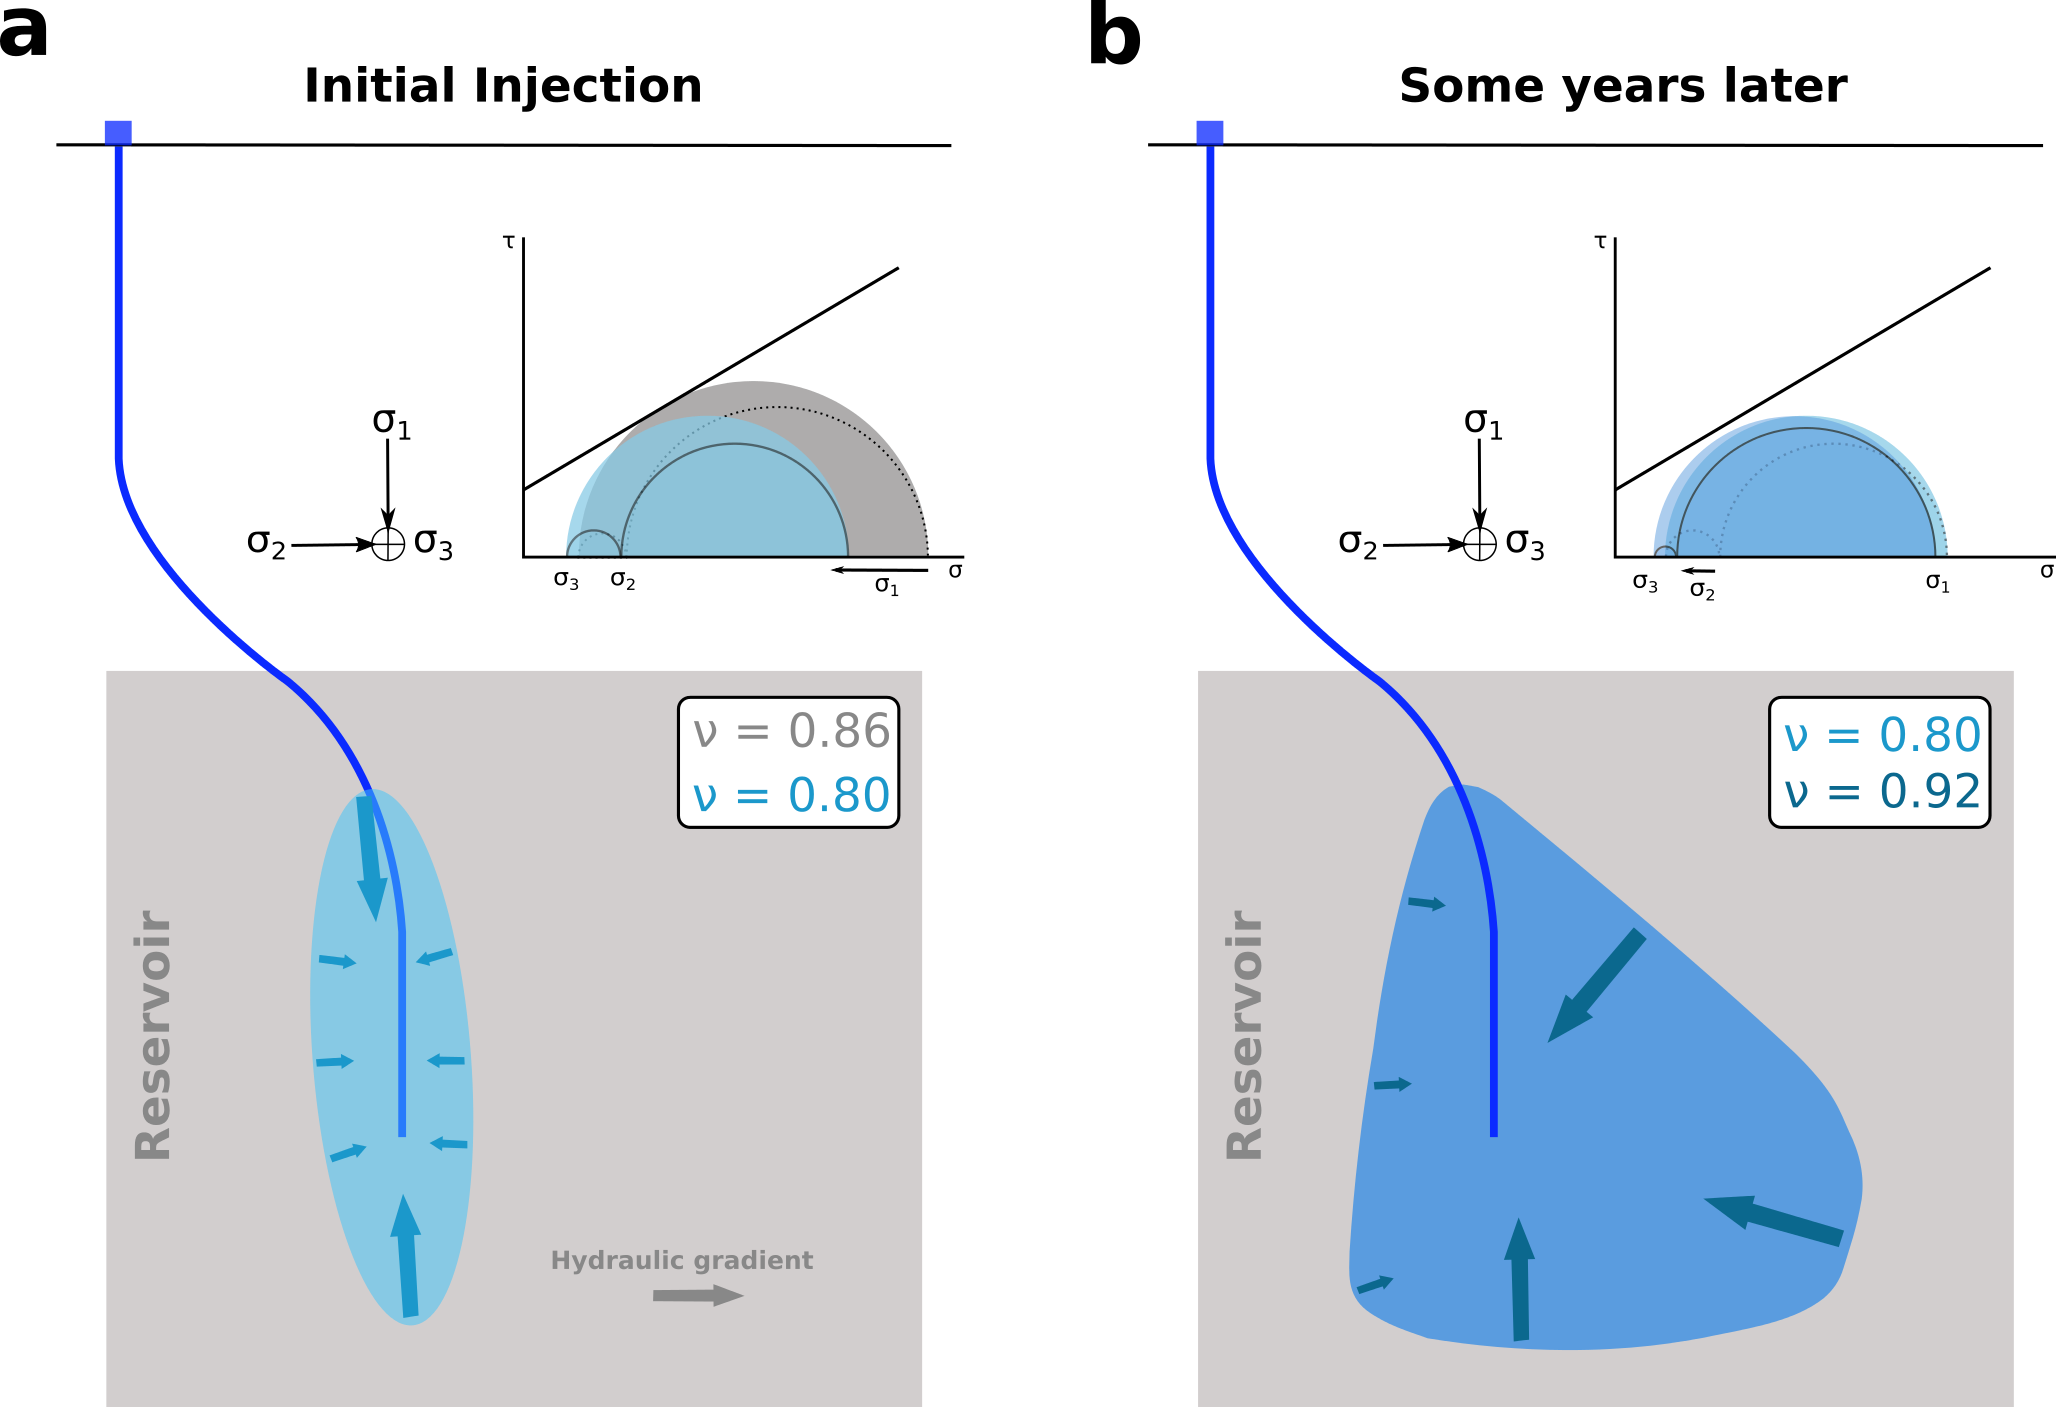
\includegraphics[width=0.65\textwidth,height=0.8\textheight,keepaspectratio]{Chapter_5_FMs/figures/cooling_schematic/res_cooling_schematic}
\caption[Effect of thermoelastic cooling on the reservoir stress state]{{
Cartoon illustrating a possible scenario for stress ratio ($\nu$) variations with time in the southeast compartment at Rotokawa. \textbf{a)} density-driven flow of cold injectate at the outset of injection, much like what may have occurred at RK23. As injection starts, the cooled zone of the reservoir is larger in the vertical dimension than in any horizontal dimension. This produces a preferential reduction of the principle stress that is most vertical. In a normal faulting regime, such as at Rotokawa, this produces a reduction of $\sigma_{1}$, as well as a reduction of differential stress and a reduction in stress ratio, $\nu$. \textbf{b)} After some years of injection (right panel), the injected fluid begins to spread laterally in the direction of greatest \gls{permeability} (i.e. subparallel to $\sigma_{2}$). As this happens, the stress reduction of $\sigma_{2}$ outpaces that of $\sigma_{1}$, the horizontal footprint of the cooled zone grows and stress ratio increases. We envision such a mechanisms to explain the oscillatory behavior of $\nu$ observed in the southeast compartment at Rotokawa, following the restart of injection at RK23. 
{\label{cooling}}%
}}
\end{center}
\end{sidewaysfigure}

If our interpretation is incorrect, and RK23-24 inject into the same pressure compartment, then it may be difficult to distinguish the contribution of each well to variations in stress. In this case, RK20 and 24 may also contribute to the temperature and pressure variations in the southeast compartment and the observed decrease in $\nu$ may also be related to the decrease in flow at RK24.

\section{Conclusions}
In this work we present 982 focal mechanisms calculated from P-wave first motion polarities for the Ngatamariki (205) and Rotokawa (777) geothermal fields in the Central Taup\={o} Volcanic Zone of New Zealand. Mechanisms at both fields are predominantly normal and strike-slip events, with small or insignificant reverse components. We have divided this catalog into various spatial and temporal clusters and inverted each for the stress tensor, seeking to determine how stress varies across the fields and assess possible relations to fluid injection activities.

Using a kmeans spatial clustering approach, we created five clusters at Ngatamariki and 14 at Rotokawa, each with a sufficient number of focal mechanisms to reliably determine the stress state from the cluster. At Ngatamariki, we show that the stress state is distinct between the northern and southern injection zones, with a normal faulting regime in the south (S$_{Hmax}\approx{}$ NE-SW) and an oblique normal faulting regime in the north with no vertical principle stresses. There are too few events at Ngatamariki to divide the catalog into meaningful temporal clusters and it is therefore difficult to comment on the effects of fluid injection on the stress state. However, it may be possible to explain the spatial variation in the stress inversions for Clusters 2 and 6 in the northern injection zone via reservoir cooling processes.

At Rotokawa, the large number of focal mechanisms (777) allows for better spatial and temporal resolution from our stress inversions. Although the stress results here show exclusively normal faulting ($\sigma_{1}\approx{\sigma_{V}}$) for all clusters, spatio-temporal variations in the direction of S$_{Hmax}$ and stress ratio, $\nu$, suggest that injection operations may be affecting the stress state. In particular, temporal variations in stress state, specifically $\nu$, for a subset of events nearest the injection wells indicate that this parameter may be sensitive to variations in injection \gls{flow_rate}. We suggest that this may reflect variations in the size and geometry of the cooled zone of the reservoir around the wells.

The findings presented here constitute the first published study of the stress variation in the Ngatamariki field and the first attempt to characterize stress from focal mechanisms at Rotokawa. The results confirm the expected first-order normal faulting regime with NE-SW S$_{Hmax}$ at both fields but show significant variation in space, especially at northern Ngatamariki where the stress field varies significantly from the south. From an operational point of view, the knowledge of the stress state away from logged wells aids in identifying the population of fractures that are well-oriented for failure, and therefore the most likely to host fluid flow. This knowledge is critical for planning injection and production strategies and for targeting wells.

\section{Appendices}
\subsection{AFIT and FMI logs}
Borehole image logs use either the variations in electrical resistivity (Formation Micro Imager: FMI) or amplitude variations in acoustic reflections off the borehole wall (AFIT: Acoustic Formation Imaging Technology) to construct an image of the well with a resolution of \textless5--10 mm \citep{massiot2015processing,McNamara_2015}. Structures intersecting the wellbore appear as sinusoids in the unwrapped image, from which the orientation of individual fractures, bedding planes and geologic contacts can be determined \citep{massiot2015processing}. For the two available FMI logs (wells NM09 and NM10), we report only `non-halo', conductive fractures as reported by \citet{nm09_report} and \citet{nm10_report}, which have the highest likelihood of being open and not filled with a sealing mineral such as pyrite or calcite. These are the strongest candidate fractures for hosting fluid flow in the reservoir, and accommodating seismic slip. The remaining logs referenced in this work were collected via AFIT, and are therefore unable to distinguish between sealed and unsealed fractures \citep{massiot_2012,massiot2015processing}. For AFIT logs, we report all fractures of both high and low confidence identified in the well log reports \citep{massiot_2012,massiot_rk18l2,massiot_rk32,mcnamara2011rk29,mcnamara2010rk30l1}.

At Ngatamariki, logs were collected at wells NM08 and NM09, in the northern injection zone, and well NM10 in the southern injection zone \citep{massiot_2012,nm09_report,nm10_report}. While the dominant strike across all wells in the field is NE-SW, dips differ between wells. Fractures in NM08 strike $\sim$030\textdegree{} and dip to the SE at an average of $\sim$65\textdegree{}, while those in NM09, $\sim$200 m to the Southeast, strike $\sim$211\textdegree{} and dip NW at $\sim$60\textdegree{}. This likely indicates the presence of antithetic structures, one intersecting NM08, dipping southeast, and the other intersecting NM09 dipping northwest \citep{massiot_2012,nm09_report}. Fractures at NM10 strike an average of $\sim$008\textdegree{} and dip $\sim$62\textdegree{} with more dipping to the southeast than northwest. There are also two subordinate strikes at NM10, one at $\sim$360\textdegree{} and another at $\sim$260\textdegree{}. The bimodal dip distribution and complex distribution of strikes likely reflect the complex structure within the Aratiatia Fault Zone, into which NM10 is drilled (Figure XX).

At Rotokawa, well logs were taken for four wells in what is now the production field: RK18L2, RK32, RK30L1 and RK29 \citep{massiot_rk18l2,massiot_rk32,mcnamara2011rk29,mcnamara2010rk30l1}. As at Ngatamariki, the majority of fractures strike NE-SW but dip in accordance with the nearest large structure (i.e. \acrshort{PFF}, \acrshort{CFF}, \acrshort{IFF}). Dips at well RK18L2, RK30L1 and RK29 are to the northwest at $\sim$69\textdegree{}, $\sim$71\textdegree{} and $\sim$68\textdegree{}, striking $\sim$199\textdegree{}, $\sim$223\textdegree{} and $\sim$161\textdegree{}, respectively. Fractures at RK32, nearest the \acrlong{PFF}, strike an average of $\sim$052\textdegree{} with a dip of $\sim$70\textdegree{}SW.

\subsection{Borehole vs focal mechanism fracture orientation}
To accompany the stress work detailed in the main body of this chapter, we have also used focal mechanism solutions to characterize the orientation of the fracture network within the area of active seismicity. This is of critical importance to geothermal operators as the orientation of open fractures reveals aspects of the flow pathways from injection to production wells. Improved understanding of these pathways allows reservoir engineers to better plan injection and production strategies in order to minimize cooling and pressure drawdown.

While focal mechanism solutions are described equally well by two orthogonal nodal planes, we can calculate which is the most likely to fail for a given stress regime. Failure increases fracture \gls{permeability} through misalignment of asperities on opposing fracture faces (a process known as self-propping). Therefore, by calculating the fractures which are best oriented for failure in a given stress regime, we are also determining the fractures which are most likely to provide pathways through which reservoir fluid will flow.

Figures \ref{237918} and \ref{237919} compare the orientations of fractures measured from borehole imaging with those inferred from the most likely failure planes from the focal mechanisms analyzed above. In order to determine which plane was the most likely to fail, we used the approach of \citet{vavryvcuk2014iterative}, who define the instability of a plane as:

\begin{equation}
I = \frac{\tau - \mu(\sigma - 1)}{\mu + \sqrt{1 + \mu^{2}}}
\end{equation}

where $\tau$ and $\sigma$ are the shear and normal tractions on a given plane, respectively and $\mu$ is the coefficient of static friction. We invert all focal mechanisms for the stress tensor at each field separately. We then use the whole-field stress result to calculate the least stable planes for each focal mechanism in the corresponding field.

% Ngatamariki fractures fig
\begin{sidewaysfigure}[p]
\begin{center}
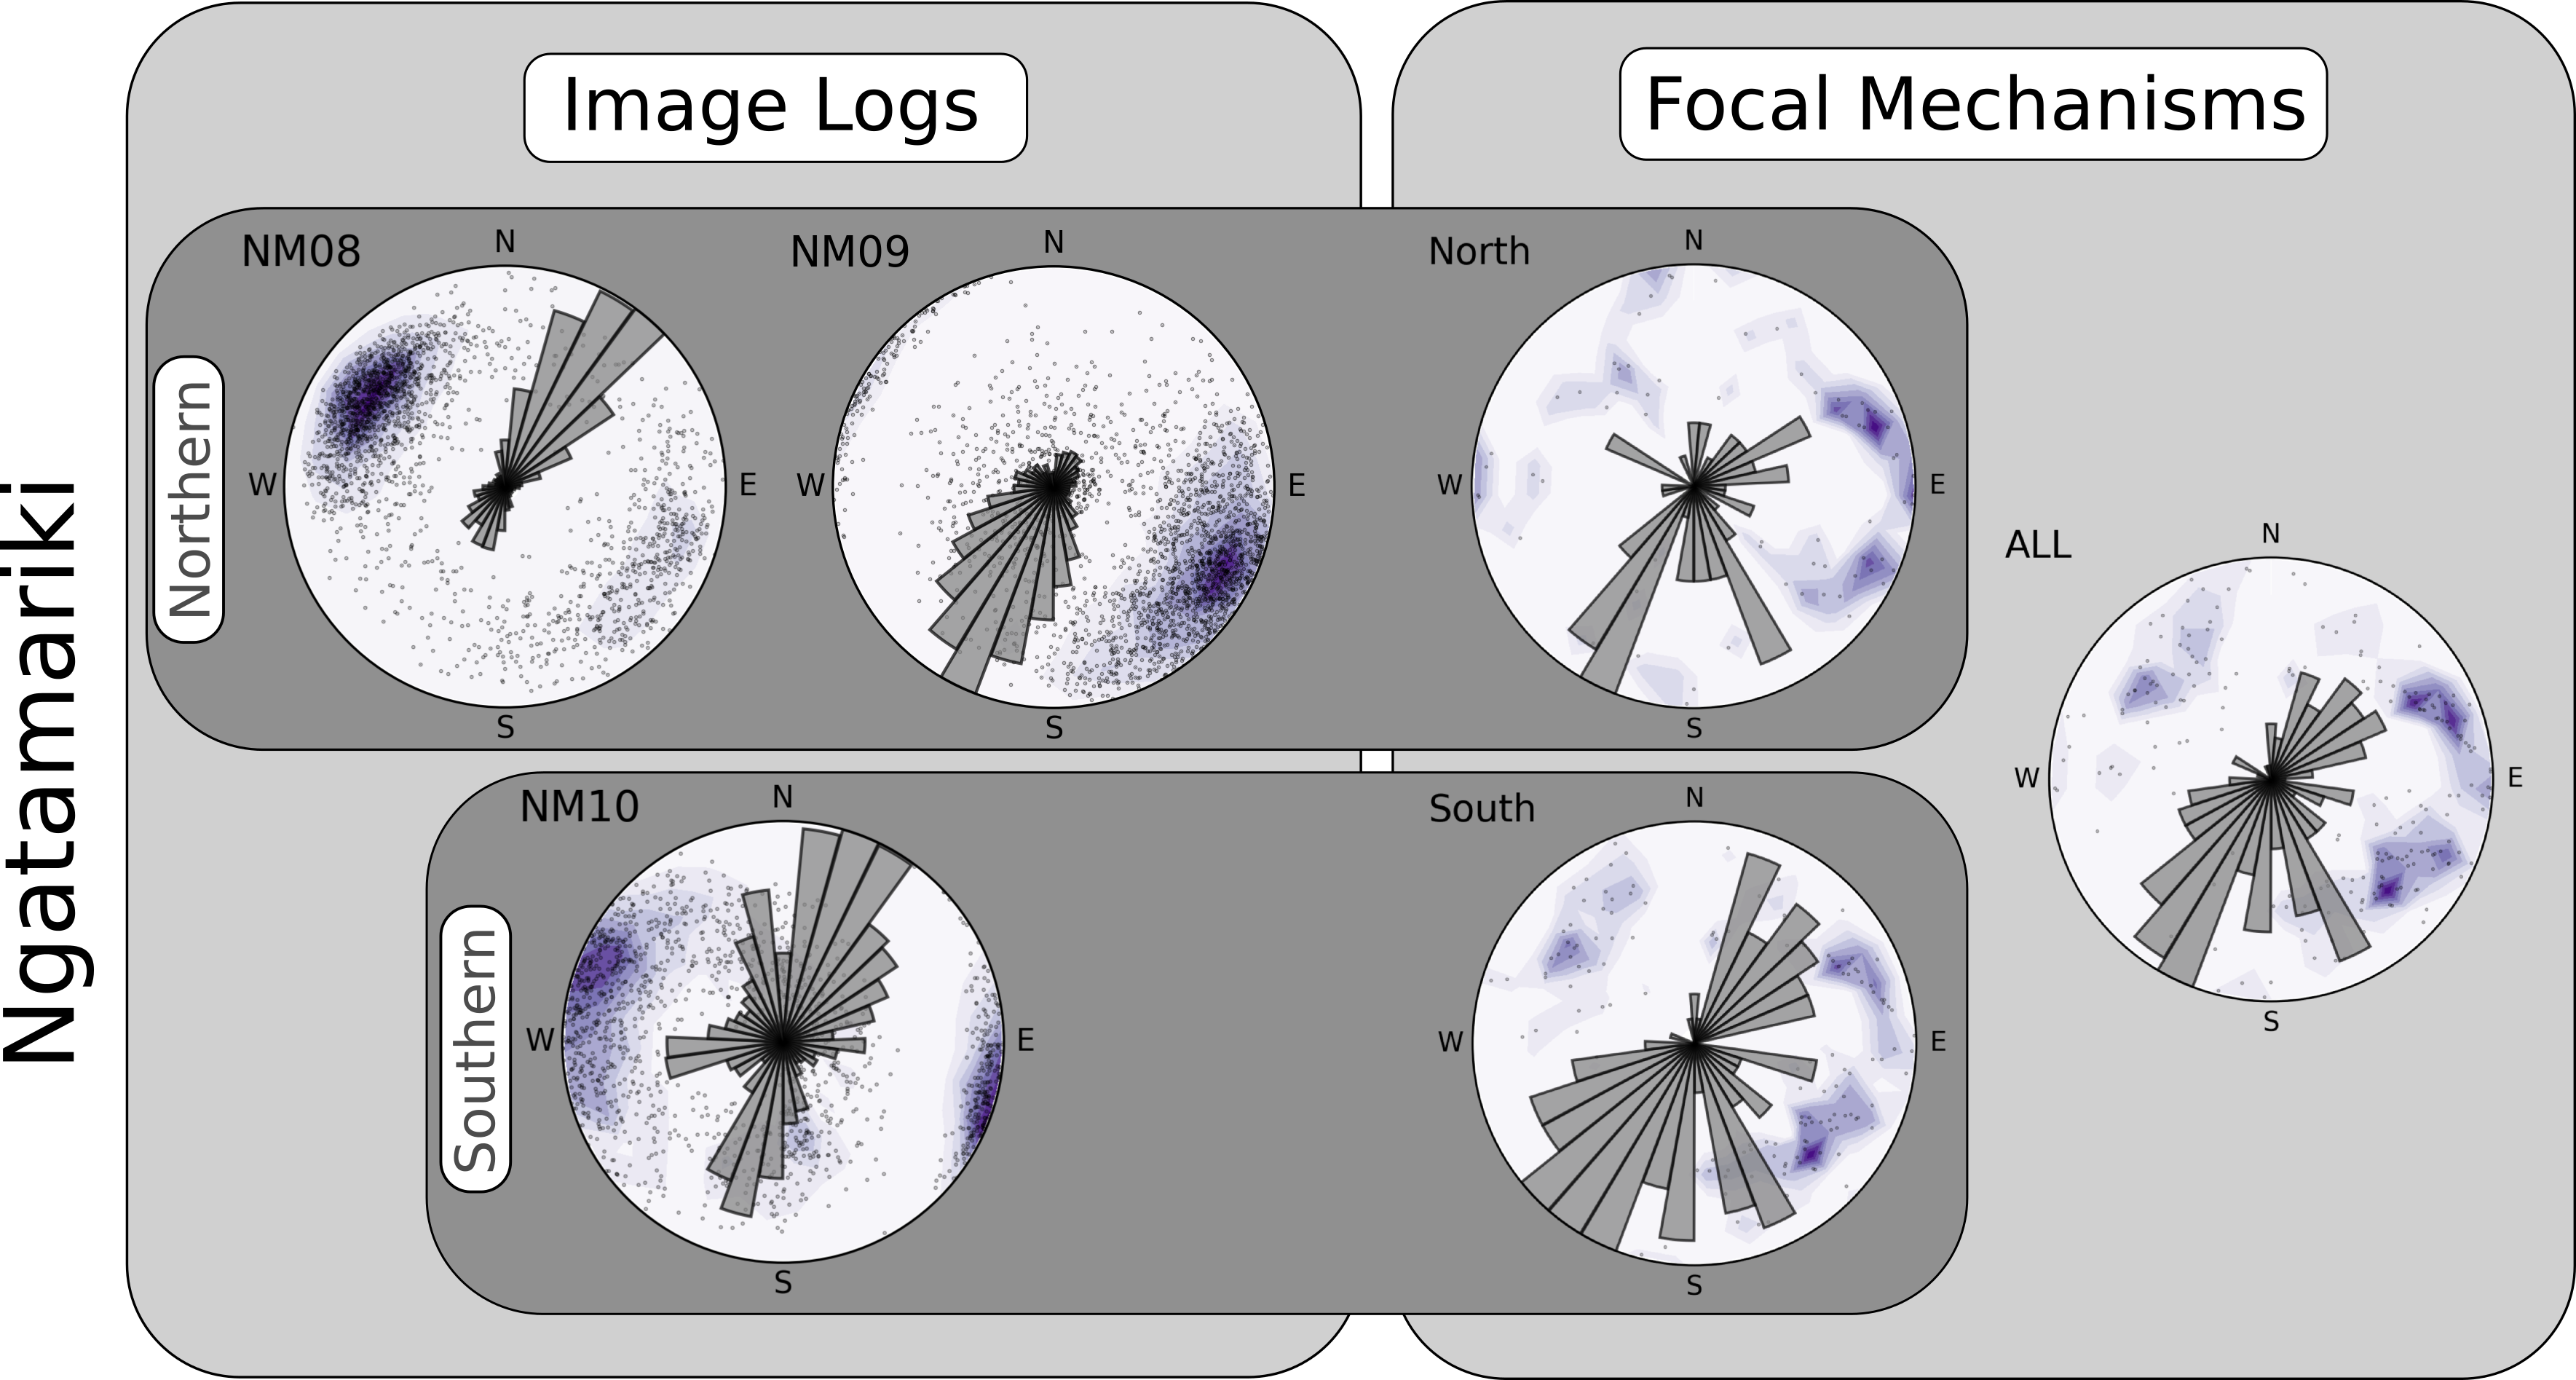
\includegraphics[width=\textwidth,height=\textheight,keepaspectratio]{Chapter_5_FMs/figures/Nga_fracture_FM/ALL_fracs_and_FMs_Ngatamariki}
\caption[Ngatamariki fracture orientations and focal mechanism nodal planes]{{
Ngatamariki fracture orientations measured from acoustic (NM08-NM09) or resistivity (NM10) imaging of boreholes, compared with the least stable nodal planes for each of the focal mechanisms in this study. The instability criterion used to decide which plane was most likely to fail was based on the approach of \citet{vavryvcuk2014iterative}.
{\label{237918}}%
}}
\end{center}
\end{sidewaysfigure}\selectlanguage{english}

In Figures \ref{237918} and \ref{237919}, we have divided both the well imaging results and focal mechanisms into the major spatial clusters for comparison. In Ngatamariki we divided the data into northern and southern injection wells and the corresponding focal mechanisms clusters (Figure \ref{237918}). The image logs for northern wells NM08 and NM09 have highly uniform fracture orientations striking NE-SW, dipping SE at NM08 and NW at NM09. The most likely nodal planes also show a preference for NE-SW strike in this portion of the reservoir, albeit mostly dipping W-NW. In northern Ngatamariki there is also a subordinate, SSE-striking, WSW-dipping population of nodal planes that do not appear in the wellbore image logs. The reasons for this discrepancy are unclear, although there is a large degree of scatter in the fracture populations measured at the wells, which means that SSE-stiking fractures do exist in the wells, albeit in relatively limited numbers.

% Rotokawa fractures fig
\begin{sidewaysfigure}[p]
\begin{center}
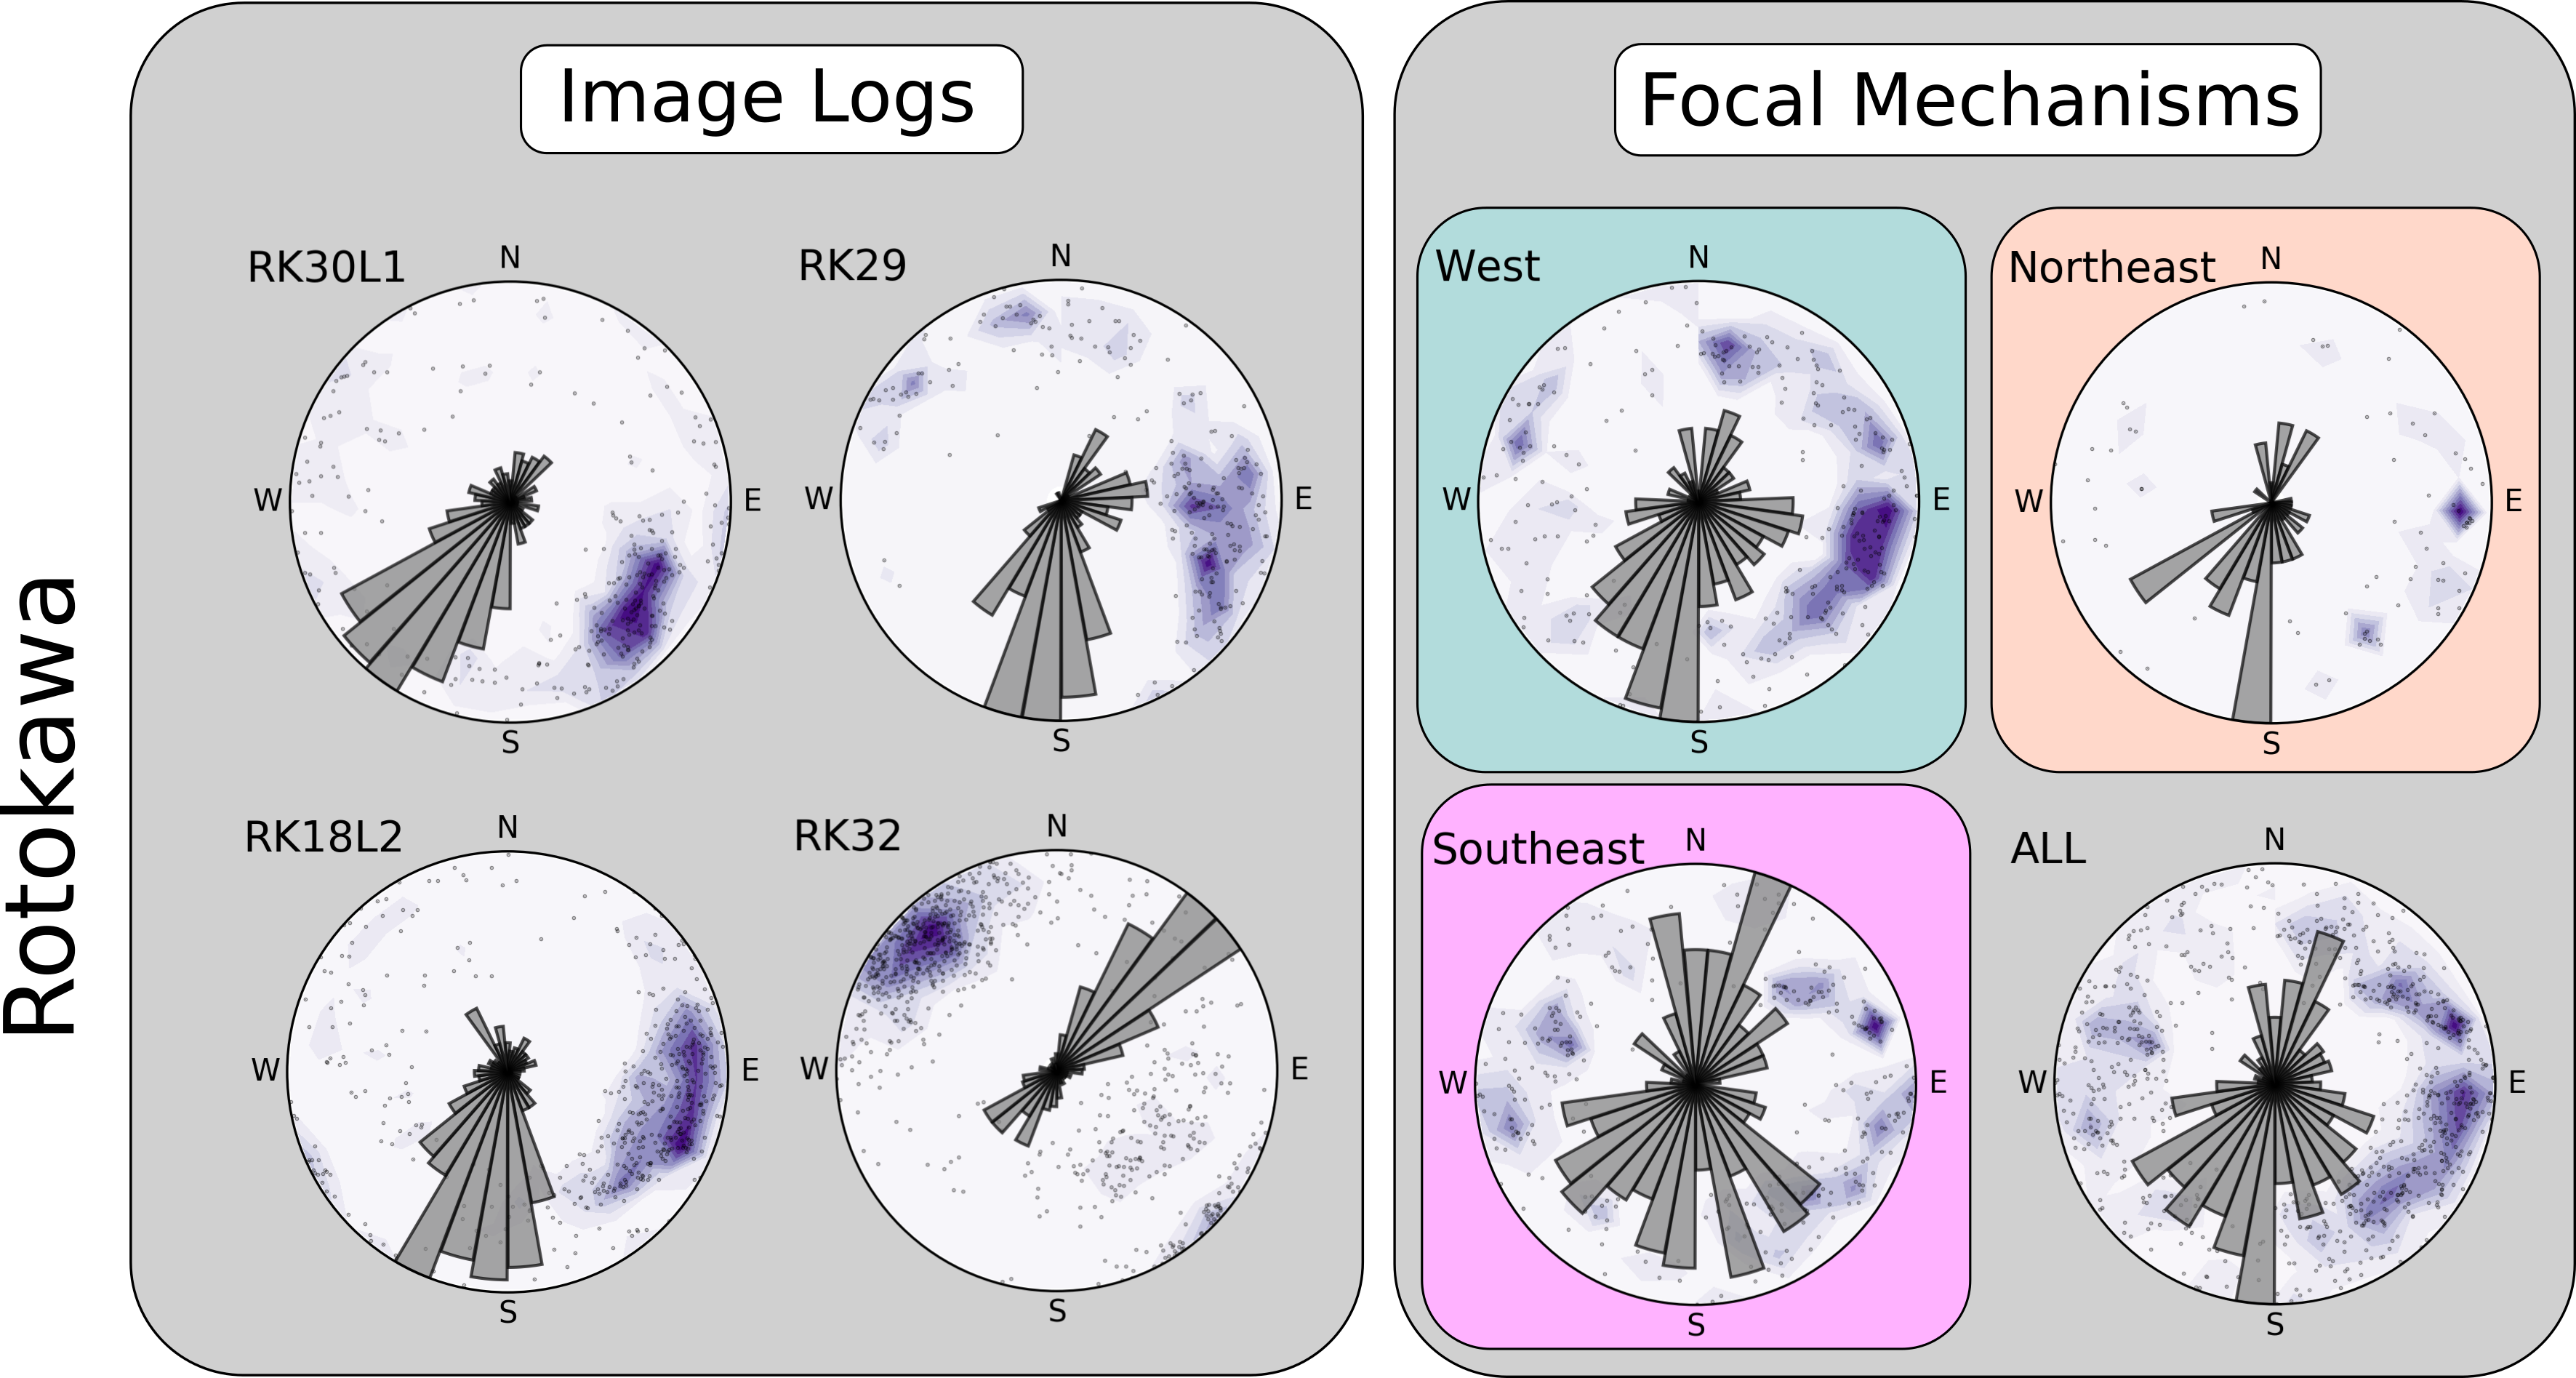
\includegraphics[width=\textwidth,height=\textheight,keepaspectratio]{Chapter_5_FMs/figures/Rot_fracture_FM/ALL_fracs_and_FMs_Rotokawa}
\caption[Rotokawa fracture orientations and focal mechanism nodal planes]{{
Rotokawa fracture orientations measured from acoustic imaging of boreholes, compared with the least stable nodal planes for each of the focal mechanisms in this study. The instability criterion used to decide which plane was most likely to fail was based on the approach of \citet{vavryvcuk2014iterative}.
{\label{237919}}%
}}
\end{center}
\end{sidewaysfigure}\selectlanguage{english}

At Rotokawa, the image logs were collected only at wells in the production field, which therefore do not correspond directly to the area of active seismicity. We divided the focal mechanisms into the western (green), southeastern (pink) and northeastern (coral) compartments discussed above and color-coded the rose plots based on the convention established in Figures \ref{878143}, \ref{434168} and \ref{533041}. For reference, the western compartment is the compartment closest to the wells for which image logs were collected (specifically RK29 and RK30L1). With that context, the image log results at RK29 and RK30L1 compare favorably with the most-likely nodal planes in the western compartment, which exhibit SSE strikes and WSW dips with small subordinate orientations of E striking, S dipping and SW-striking, NW-dipping fractures and nodal planes. Although it contains fewer focal mechanisms and is located further from the logged wells, the northeast compartment exhibits a similar nodal plane distribution to the western compartment. In contrast, the southeast compartment shows a much wider distribution of likely nodal plane orientations with a dominant orientation of NNE-striking, ESE-dipping fractures. We interpret this well-distributed population of unstable fractures as an indication of elevated pore-pressures in this injection-adjacent compartment of the reservoir. Elevated pore pressures should have the effect of broadening the distribution of fractures that are critically stressed in a given stress regime, which has been suggested for injection operations elsewhere \citep[e.g.][]{Bachmann_2012}. We think this approach to fracture network characterization can be applied to sets of focal mechanisms at geothermal reservoir elsewhere and paired with the stress determination detailed above to better understand the orientation of flowing fractures and \gls{permeability} away from wells.